\chapter{مفاهیم پایه و نگاهی بر کارهای پیشین}

\section{مفاهیم پایه}
برای آنکه درک مناسبی از مسئله‌ پیاده‌سازی دوقلوی دیجیتال و تشخیص اجسام پویا ایجاد شود، نیاز است که ابزار‌ها و الگوریتم‌هایی که در این پژوهش از آنها استفاده شده است به صورت اجمالی تعریف شوند.

\subsection{حسگرها}
حسگرها به عنوان اجزای ضروری در عرصه فناوری و جمع‌آوری داده‌ها، به عنوان چشم‌ها و گوش‌های سیستم‌های مختلف عمل می‌کنند. این دستگاه‌های الکترونیکی برای تشخیص و پاسخ به تغییرات فیزیکی یا محیطی طراحی شده‌اند و ظواهر جهان واقعی را به داده‌های قابل اندازه‌گیری تبدیل می‌کنند. حسگرها انواع گوناگونی دارند؛ از حسگرهای دما که تغییرات حرارتی را نظارت می‌کنند تا حسگرهای حرکت که حرکت را تشخیص می‌دهند. آنها در بسیاری از کاربردها مورد استفاده قرار می‌گیرند، از سیستم‌های خودرویی که ایمنی وسیله نقلیه را تضمین می‌کنند تا دستگاه‌های خانه هوش مصنوعی که راحتی و کارایی را افزایش می‌دهند. با توانایی در تجزیه و تحلیل داده‌ها به صورت بلادرنگ، حسگرها نقش اساسی در زمینه‌هایی مانند بهداشت، تولید، نظارت بر محیط زیست و موارد دیگر ایفا می‌کنند و تصمیم‌گیری آگاهانه و خودکارسازی فرآیندهای مختلف را در دنیای متصل ما امکان‌پذیر می‌سازند.

\subsubsection{حسگر لایدار}
لایدار یک اختصار برای تشخیص و فاصله‌سنجی با نور\LTRfootnote{\lr{LiDAR = Light Detection and Ranging}} است. در لایدار، نور لیزر از یک منبع (فرستنده) ارسال می‌شود و از اجسام حاضر در صحنه بازتاب می‌یابد. نور بازتاب شده توسط گیرنده سیستم تشخیص داده می‌شود و از زمان پرواز\LTRfootnote{\lr{TOF: Time of Flight}} این نور، برای توسعه نقشه فاصله\LTRfootnote{\lr{Distance Map}} اجسام استفاده می‌شود \cite{Synopsis:LiDAR}.


به طور اصولی، لایدار یک دستگاه اندازه‌گیری فاصله به هدف است که با ارسال یک پالس کوتاه نوری و ثبت زمان گذشته بین پالس نوری خروجی و تشخیص پالس نوری بازتابی (برگشتی)، فاصله را اندازه‌گیری می‌کند.

\begin{figure}[h]
	\centering
	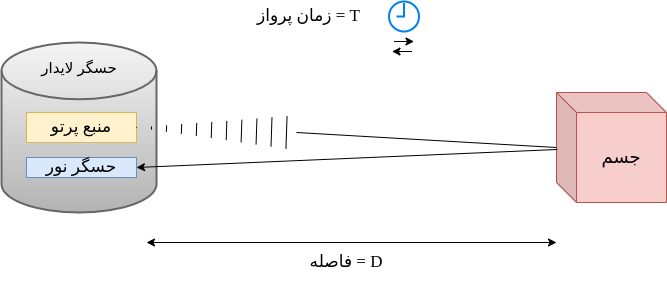
\includegraphics[scale=0.5]{figures/LiDAR_TOF.png}
	\caption{تصویری از نحوه محاسبه فاصله اجسام توسط حسگر لایدار}
	\label{fig:LiDAR_TOF}
\end{figure}

طبق \cref{fig:LiDAR_TOF}، با دانستن سرعت نور که با \lr{c} نمایش داده می‌شود داریم:
\begin{equation}\label{d=ct/2}
d = c \cdot t / 2
\end{equation}

یک سیستم لایدار ممکن است از آینه اسکن\LTRfootnote{\lr{Scan Mirror}}، چند پرتو لیزر یا ابزارهای دیگر برای اسکن فضای شیء استفاده کند. با توانایی ارائه اندازه‌گیری دقیق فواصل، لایدار می‌تواند برای حل مسائل متنوعی مورد استفاده قرار گیرد.

در حوزه حسگری از دور\LTRfootnote{\lr{Remote Sensing}}، سیستم‌های لایدار برای اندازه‌گیری پراکندگی، جذب یا بازتاب از ذرات یا مولکول‌های موجود در جو استفاده می‌شوند. برای این اهداف، سیستم‌ها ممکن است نیازهای خاصی در خصوص طول موج پرتوهای لیزری داشته باشند. می‌توان غلظت یک گونه مولکولی خاص در جو، به عنوان مثال متان و بار آئروسل\LTRfootnote{\lr{Aerosol Loading}} را اندازه‌گیری کرد. همچنین قطرات باران در جو می‌توانند اندازه‌گیری شوند تا فاصله یک توفان و نرخ بارندگی را تخمین بزنند.

سیستم‌های دیگر لایدار محور، مشخصات سطوح سه‌بعدی در فضای جسمی\LTRfootnote{\lr{Object Space}} را ارائه می‌دهند. در این سیستم‌ها، پرتوهای لیزری طیف خاص و مشخصی ندارند. به جای آن، ممکن است طول موج پرتوهای لیزری برای اطمینان از ایمنی چشمی یا جلوگیری از ویژگی‌های طیفی جو انتخاب شود. پرتوی مورد ارزیابی برخورد کرده و توسط یک "هدف سفت" به سمت گیرنده لایدار بازتاب می‌شود.

\begin{figure}[h]
    \centering
    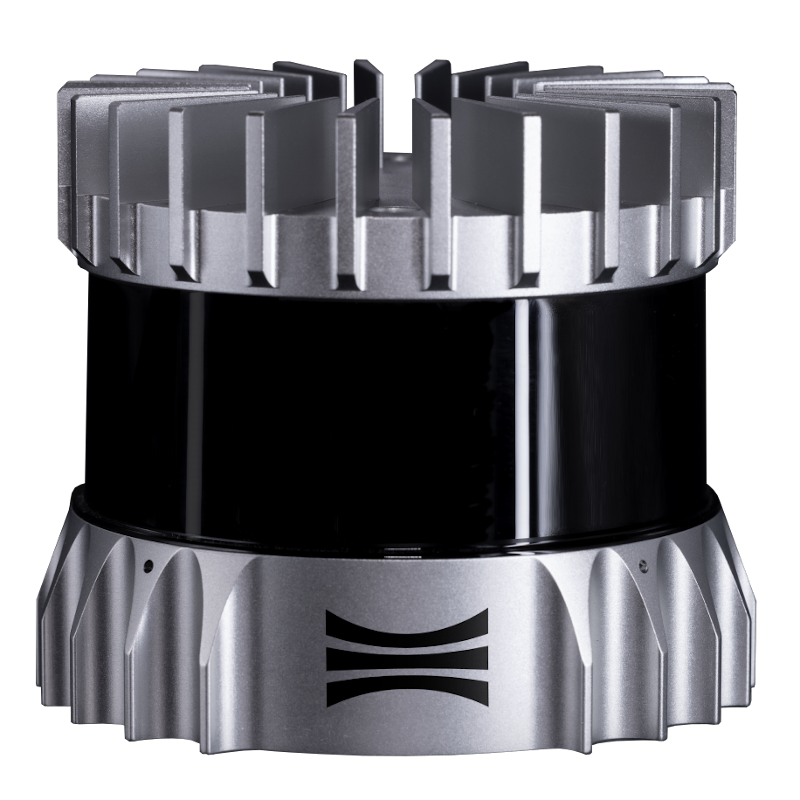
\includegraphics[width=0.25\linewidth]{figures/OS1_64_LiDAR.png}
    \caption{حسگر لایدار \lr{OS1:64} از شرکت \lr{Ouster} \cite{Ouster:LiDAR_Specification}}
    \label{fig:OS1_64_LiDAR}
\end{figure}

لایدار همچنین می‌تواند برای تعیین سرعت یک جسم هدف، مورد استفاده قرار گیرد. این کار می‌تواند به وسیله تکنیک داپلر\LTRfootnote{\lr{Doppler Technique}} یا اندازه‌گیری فاصله تا یک هدف در مدت زمان کوتاهی انجام شود. به عنوان مثال، سرعت باد جوی و سرعت یک خودرو می‌تواند توسط یک سیستم لایدار اندازه‌گیری شود.

علاوه بر این، سیستم‌های لایدار می‌توانند برای ایجاد مدل سه‌بعدی از یک صحنه پویا مورد استفاده قرار گیرند، همانند صحنه‌هایی که یک خودروی خودران با آن مواجه می‌شود. این کار در روش‌های مختلفی قابل انجام است اما معمولاً با استفاده از تکنیک‌های اسکن‌کردن ۳۶۰ درجه و محسابه زمان پرواز صورت می‌گیرد.

در حال حاضر، به طور متداول برای ایجاد مدل سه‌بعدی از دنیای اطراف حسگر لایدار مورد استفاده قرار می‌گیرد. سیستم‌های مسیریابی خودکار از سیستم‌هایی است که از ابر نقاط ایجاد شده توسط حسگر لایدار استفاده می‌کند. برخلاف تصاویر، ابر نقاط پراکنده هستند: نمونه‌ها به طور یکنواخت در فضا توزیع نشده‌اند. لایدارها به عنوان حسگرهای فعال، نیازی به نور محیطی ندارند و از این رو می‌توان با توجه به شرایط آب و هوایی نامساعد، تشخیص قابل اعتمادتری انجام داد \cite{arnold2019survey}. سیستم‌های کوچکتر لایدار حتی در دستگاه‌هایی با اندازه‌های کوچک مانند تلفن‌های همراه نیز یافت می‌شوند.

\subsubsection{دستگاه \lr{RSU}}
\lr{RSU}\LTRfootnote{\lr{Roadside Unit}}یک گیرنده و فرستنده است که عموما در کنار خیابان‌ها و خطوط عابرپیاده مستقر می‌شود. این دستگاه‌ها می‌توانند بر روی یک خوردرو نیز مستقر شوند و یا با دست حمل شوند اما تنها زمانی شروع به کار کردن می‌کند که ثابت باشد و در حال حرکت نباشد. \lr{RSU}ها تنها در منطقه‌ای که مجوز آن‌ را داشته باشند می‌توانند عمل کنند. اما آنهایی که توسط دست نیز حمل می‌شوند، می‌توانند بدون مجوز در منطقه‌هایی که تداخلی با بقیه \lr{RSU}های دارای مجوز و دولتی ندارند، عمل کنند. این دستگاه‌ها داده‌‌های ترافیکی و آب‌وهوایی را به سیستم‌های مدیریت کلان شهری می‌فرستند و همچنین از آنها اطلاعات می‌گیرند. همچنین دستور‌هایی را می‌توانند به ماشین‌ها بدهند تا از خطر احتمالی و یا  ترافیک احتمالی جلوگیری شود. در این پژوهش منظور از \lr{RSU}،  حسگر لایداری است که در کنار خیابان مستقر شده است.

\subsection{شبکه‌های عصبی}
یادگیری ماشین\LTRfootnote{Machine Learning (ML)} یک روش موثر برای رسیدن به اهداف هوش‌مصنوعی است و روش‌های متعددی برای آموزش ماشین جهت دسته‌بندی و پیش‌بینی ارائه شده است. در میان این روش‌ها، یادگیری عمیق با استفاده از شبکه‌ی عصبی به نتایج فوق‌العاده‌ای در انواع کارها مانند پردازش تصویر، تشخیص چهره و غیره دست‌ یافته است. شبکه‌ی عصبی مجموعه‌ای از الگوریتم‌ها است که تلاش می‌کند تا روابط زیربنایی را در مجموعه‌ای از داده‌ها از طریق فرایندی که نحوه‌ی عملکرد مغز انسان را تقلید می‌کند، تشخیص دهد \cite{zhou2019edge}. 

از آن جا که شبکه‌ی عصبی\LTRfootnote{Neural Networks} در یادگیری عمیق، شامل چندین لایه است، به آن شبکه‌ی عصبی عمیق اطلاق می‌شود. همان‌طور که در \cref{fig:standard_nn} مشاهده می‌شود هر لایه در شبکه‌ی عصبی عمیق از نورون‌هایی تشکیل شده است که قادرند بر اساس داده‌ی ورودی، خروجی غیرخطی تولید نمایند.

\begin{figure}[h]
    \centering
	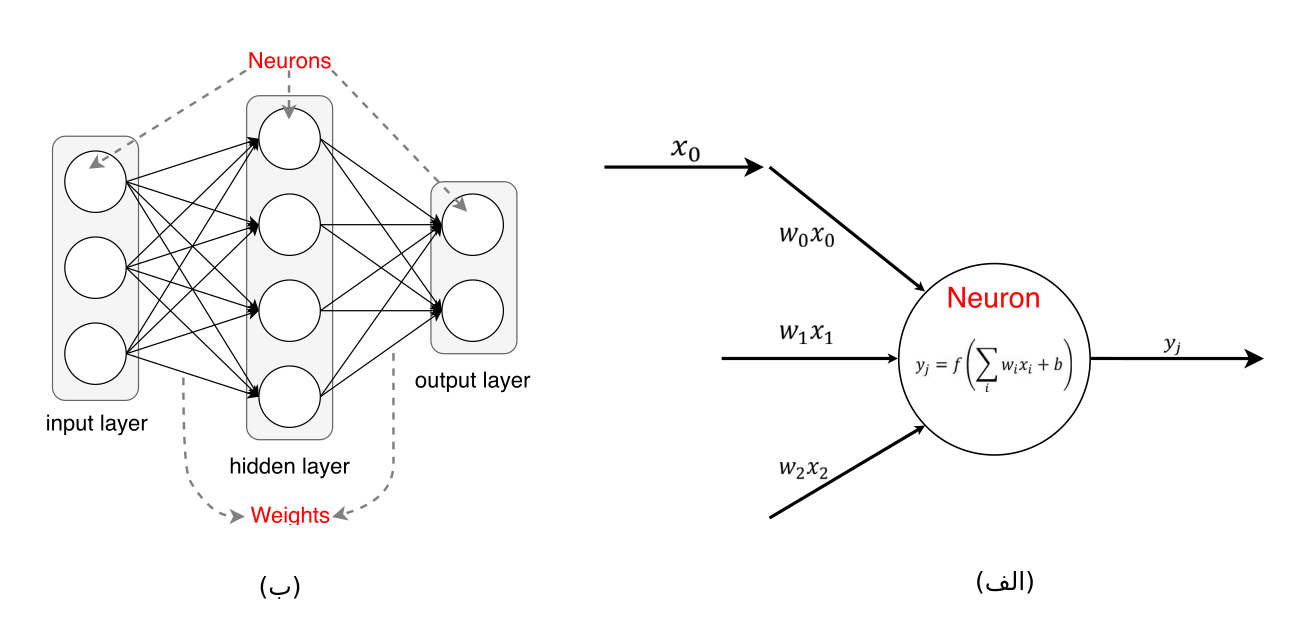
\includegraphics[width=1\linewidth]{figures/standard_nn.png}
	\caption{مدل استاندارد شبکه‌ی عصبی عمیق \cite{zhou2019edge}}
	\small\textsuperscript{عصبی عمیق شبکه‌ی لایه‌های (ب) نورون یک معماری (الف)}
	\label{fig:standard_nn}
\end{figure}

\subsubsection{شبکه‌های عصبی پیچشی}

شبکه‌های عصبی پیچشی\LTRfootnote{Convolutional Neural Network (CNN)} یا به‌اختصار شبکه‌های پیچشی، دسته‌ای از شبکه‌های عصبی مصنوعی هستند که از دیگر شبکه‌های عصبی در کاربردهایی با ورودی‌های سیگنال تصویر، گفتار یا صوتی عملکرد بهتری نشان می‌دهند و معماری آن‌ها از سازمان‌دهی قشر بینایی حیوانات الهام گرفته شده است.  در این مدل، لایه‌ها با استفاده از تابع پیچش\LTRfootnote{\lr{Convolution}}، ویژگی‌های ساده ورودی را استخراج می‌کنند. فیلترهای پیچشی در این مدل سهم زیادی در نمایش سطح بالای داده‌های ورودی داشته‌اند و در این معماری شبکه مستقیما از داده‌ها یاد می‌گیرد و نیاز به استخراج دستی ویژگی را از بین می‌برد. یک نمونه از این شبکه‌ها که برای طبقه‌بندی عکس از آن استفاده شده است در \cref{fig:standard_cnn} قابل ‌مشاهده است. این نوع شبکه‌ی عصبی معمولا دارای سه ‌لایه‌ی اصلی است که عبارت‌اند از: 

\begin{enumerate}
	\item لایه‌ی پیچش
	
	\item لایه‌ی ادغام\LTRfootnote{\lr{Pooling Layer}}
	
	\item لایه‌ی تماما متصل\LTRfootnote{\lr{Fully-connected Layer}}
\end{enumerate}

\begin{figure}[h]
    \centering
    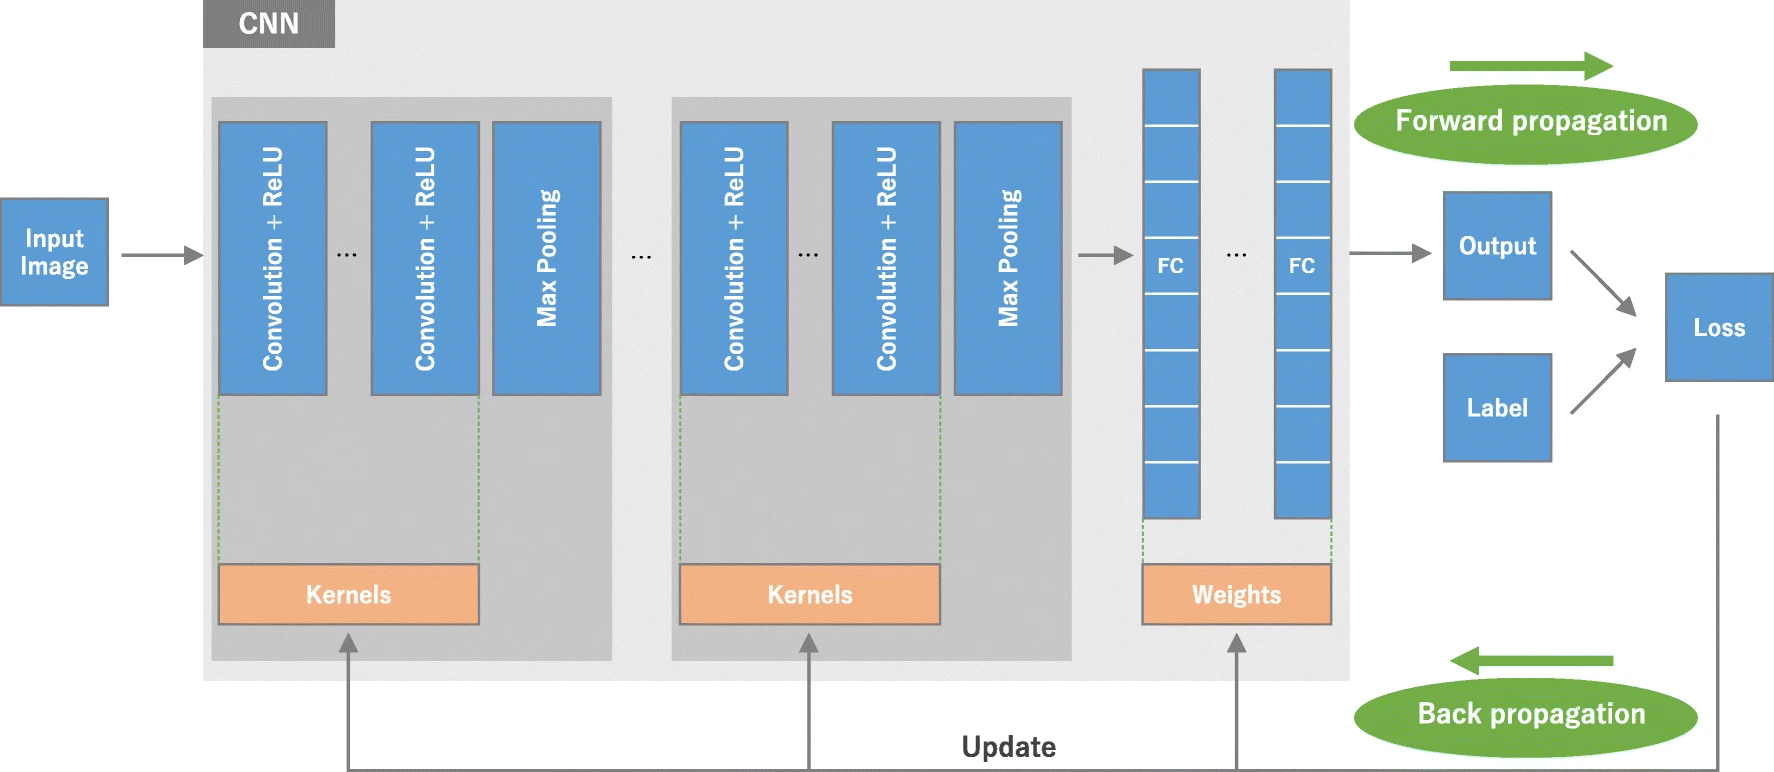
\includegraphics[width=1\linewidth]{figures/standard_cnn.png}
    \caption{نگاهی کلی به معماری استاندارد شبکه‌های پیچشی \cite{yamashita2018convolutional}}
    \label{fig:standard_cnn}
\end{figure}

دو لایه‌ی اول و دوم که لایه‌های پیچش و ادغام هستند، استخراج ویژگی را انجام می‌دهند. در حالی که لایه‌ی سوم، ویژگی‌های استخراج شده را در خروجی نهایی، نگاشت می‌کند یا به عبارتی دیگر از ویژگی‌های استخراج شده، استنتاج می‌کند. لایه‌ی پیچشی نقش کلیدی را در شبکه‌های پیچشی ایفا می‌کند، که از مجموعه‌ای از  عملیات ریاضی، نظیر پیچش تشکیل شده است \cite{yamashita2018convolutional}.

\subsubsection{لایه‌ پیچش}

 لایه پیچش از اجزای اساسی معماری شبکه‌های عصبی پیچشی است که عملیات استخراج ویژگی را انجام می‌دهد. این عملیات به طور معمول شامل ترکیبی از عملیات خطی و غیرخطی، یعنی عملیات پیچش و تابع فعال‌سازی می‌شود.

پیچش یک عملیات ویژه خطی است که برای استخراج ویژگی‌ها استفاده می‌شود. در این عملیات، یک ماتریس کوچک از اعداد به نام هسته یا فیلتر\LTRfootnote{\lr{Kernel (Filter)}}، بر روی ورودی اعمال می‌شود. ورودی نیز یک ماتریس از اعداد به نام تنسور\LTRfootnote{\lr{Tensor}} است. با قرار گرفتن فیلتر بر روی هر بخش از تنسور، اعداد فیلتر درایه به درایه در مولفه‌های تنسور متناظر ضرب می‌شوند و در نهایت همه اعداد با هم جمع می‌شوند تا یک نقشه ویژگی\LTRfootnote{\lr{Feature Map}} شکل بگیرد. اگر یک تنسور دوبعدی از یک تصویر به نام \lr{I} و یک فیلتر به نام \lr{k} داشته باشیم، عملیت پیچش طبق فرمول زیر انجام می‌شود:
\begin{equation}
    \sum_{m}\sum_{n} i(m, n)k(i-m, j-n)
\end{equation}
این پروسه با فیلترهای مختلف تکرار می‌شود که هر کدام ویژگی‌های مختلفی از تنسور را استخراج می‌کنند.\begin{figure}[h!]
    \begin{minipage}{0.5\textwidth}
        \centering
        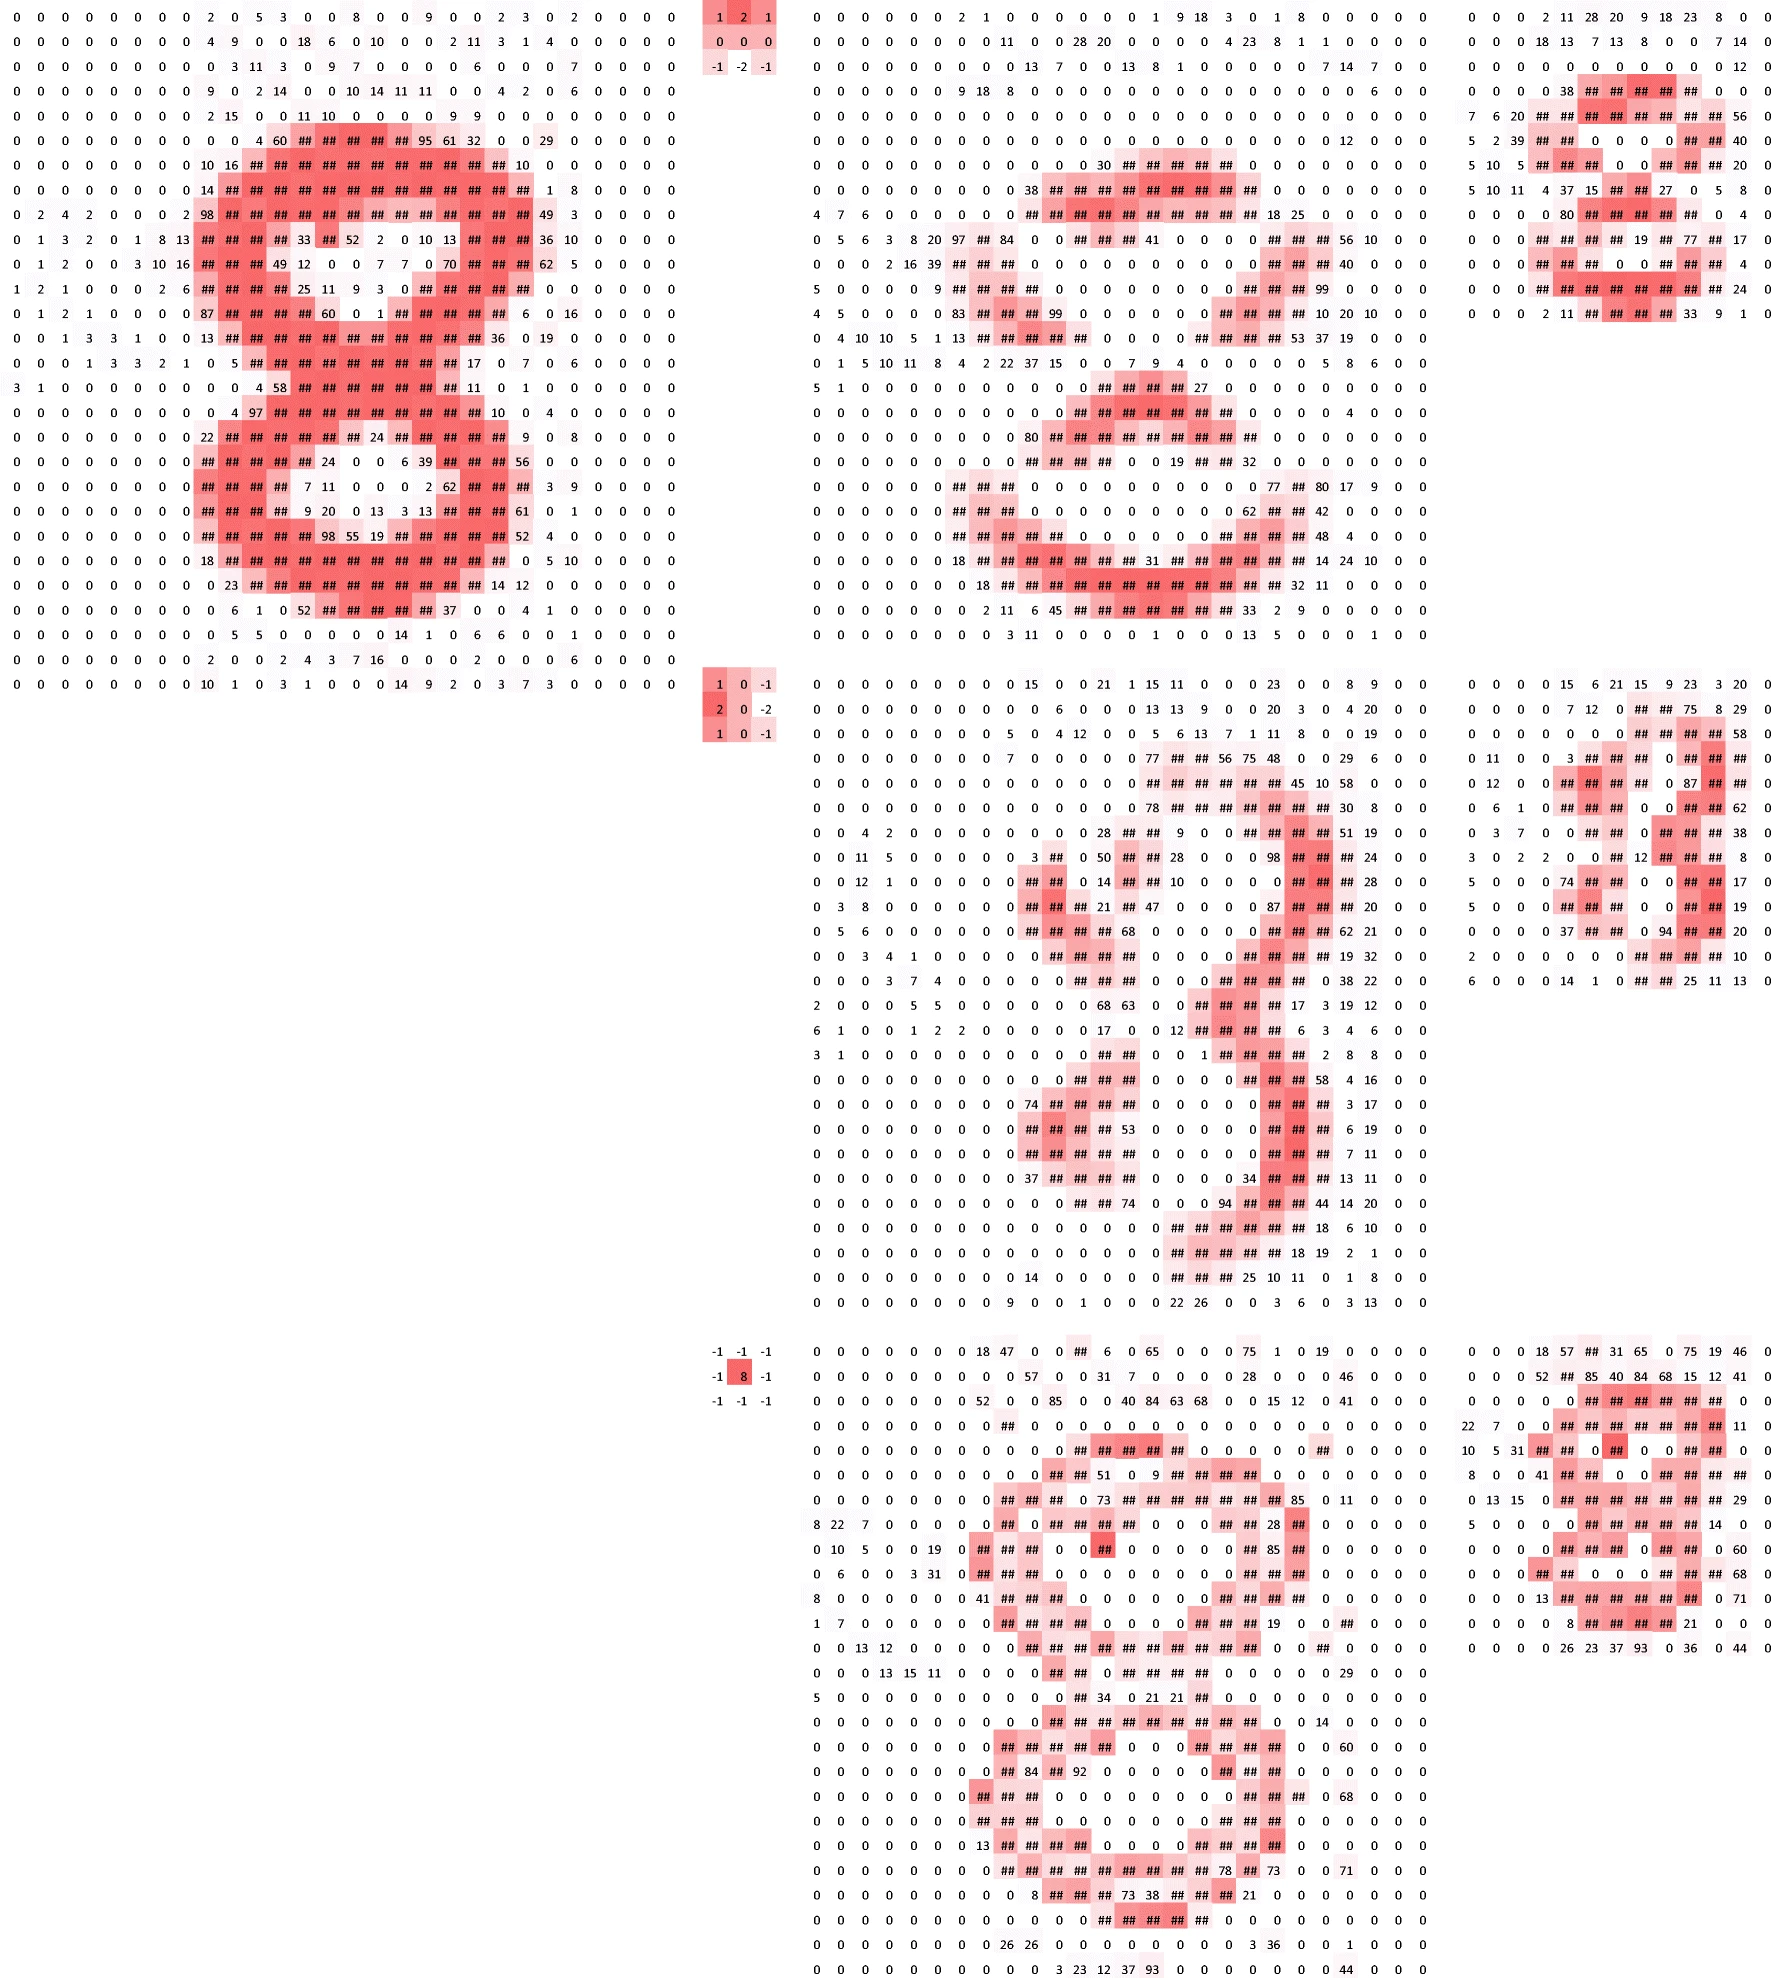
\includegraphics[width=1\linewidth]{figures/Feature_Map.png}
    \end{minipage}
    \hspace{0.3cm}
    \begin{minipage}{0.5\textwidth}
        \centering
        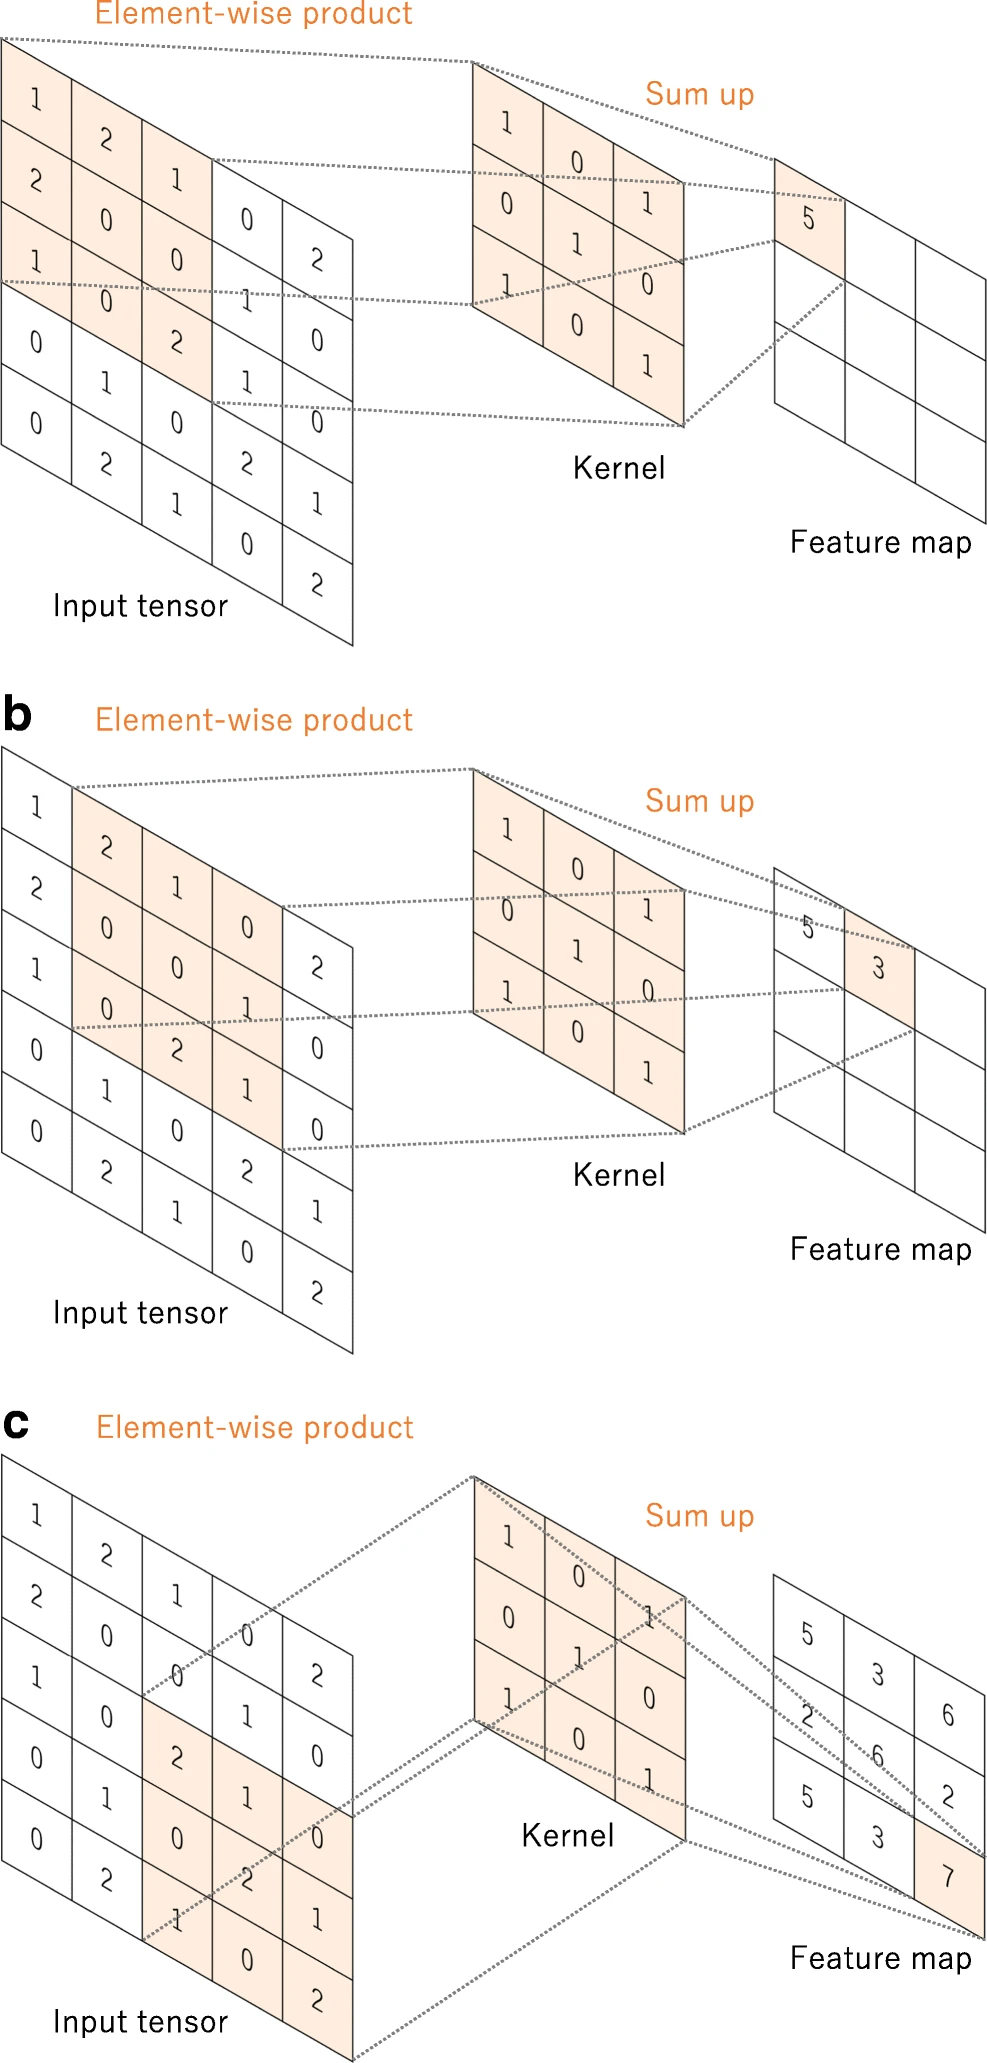
\includegraphics[width=0.9\linewidth]{figures/Convolution_Procedure.png}
    \end{minipage}
    \begin{center}
        \caption{عملیت پیچش با فیلترهای ۳ $\times$ ۳ و گام‌ ۱ \cite{yamashita2018convolutional}}
        \small\textsuperscript{می‌کنیم. مشاهده را مختلف فیلترهای ویژگی نقشه‌های شکل،  راست سمت در}
    \end{center}
    \label{fig:convolution_procedure}
\end{figure} ابرپارامتر‌هایی\LTRfootnote{\lr{Hyperparameter}} که نتیجه عملیات پیچش را تحت تاثیر قرار می‌دهند، ابعاد و تعداد ماتریس‌های فیلتر است. عموما ابعاد فیلترها ۳ $\times$ ۳ است، اما بعضی اوقات از ابعاد ۵ $\times$ ۵ و ۷ $\times$ ۷ نیز استفاده می‌شود. تعداد فیلترها عموما دلخواه است و عمق نقشه‌های ویژگی را تحت تاثیر قرار می‌دهد.

عملیات پیچشی که در \cref{fig:convolution_procedure} دیده‌ می‌شود، نمی‌گذارد که ماتریس فیلتر از ماتریس تنسور خارج شود. در واقع نقطه مرکز فیلتر هیچ‌گاه بر روی درایه‌های گوشه‌ای تنسور قرار نمی‌گیرد. این باعث می‌شود که ابعاد نقشه‌ی ویژگی‌ حاصل، کوچک‌تر از ابعاد تنسور باشد. لایه‌گذاری‌\LTRfootnote{\lr{Padding}}، که معمولا لایه‌گذاری صفر‌\LTRfootnote{\lr{Zero Padding}} است، یک روش برای حل این مشکل است. در این روش سطرها و ستون‌های تماما صفر به دور ماتریس تنسور اضافه می‌شوند. با این کار، مرکز فیلتر بر روی مولفه‌های گوشه ماتریس نیز جای می‌گیرد و نقشه ویژگی حاصل، هم‌اندازه تنسور خواهد شد. عموم مدل‌های عمیق شبکه‌های پیچشی، از لایه‌های پیچش زیادی استفاده می‌کنند و اگر از تکنیک لایه‌گذاری صفر استفاده نکنند، نقشه ویژگی آنها کوچکتر و کوچکتر می‌شود و عملا بدرد نخواهد خورد.

\begin{figure}[h!]
    \centering
    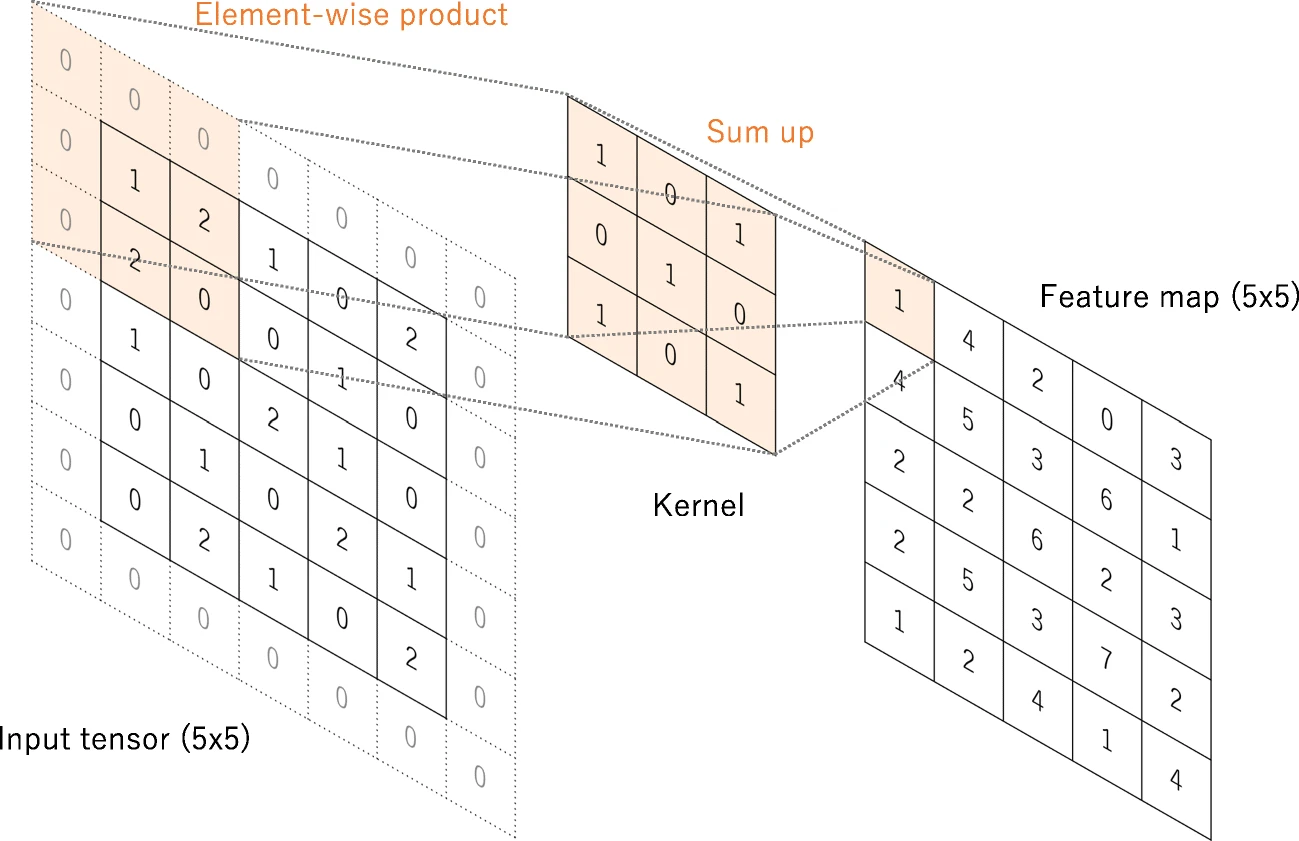
\includegraphics[width=1\linewidth]{figures/Zero_Padding.png}
    \caption{یک عملیات پیچش با لایه‌گذاری صفر \cite{yamashita2018convolutional}}
    \label{fig:zero_padding}
\end{figure}

طبق \cref{fig:zero_padding}، مشاهده می‌کنیم که با لایه‌گذاری صفر، ابعاد نقشه ویژگی هم اندازه تنسور ورودی است. اما بایستی دقت کرد که برای فیلتر‌های بزرگ‌تر و گام‌های\LTRfootnote{\lr{Stride}} بیشتر، نیاز به لایه‌گذاری صفر بیشتری خواهیم داشت. به فاصله بین دو عملیات اعمال فیلتر در یک سطر را گام می‌گویند. اندازه گام عموما ۱ است، اما گام‌های بیشتر از ۱ نیز در مواقعی که نیاز به نمونه‌کاهی\LTRfootnote{\lr{Downsampling}} نقشه ویژگی باشد، استفاده می‌شود. عملیات پیچش سه‌بعدی نیز به همین شکل است با این تفاوت که فیلترها سه‌بعدی هستند و در راستای عمق تنسور سه‌بعدی ورودی نیز حرکت می‌کنند.
\\
شبکه‌های عصبی پیچشی، دارای دامنه‌ی گسترده‌ای از کاربردها هستند و به خارج از تشخیص تصویر\LTRfootnote{\lr{Image Recognition}} گسترش یافته‌اند. از یادگیری سلسه‌وار ویژگی‌های آنها نیز در پردازش زبان طبیعی\LTRfootnote{\lr{Natrual Language Processing (NLP)}} و تجزیه و تحلیل گفتار\LTRfootnote{\lr{Speech Recogntion}} بهره‌برداری می‌شود. علاوه بر این، شبکه‌های عصبی پیچشی جلو‌دار تازه‌ترین پیشرفت‌ها در خودروهای خودران بوده‌اند، جایی که داده‌ها از حسگرهایی مانند لایدار و دوربین‌ها پردازش می‌شود، تا تصمیم‌گیری بلادرنگ در سناریو‌های مختلف رانندگی را ممکن کند. با توسعه مداوم معماری‌های شبکه‌های عصبی پیچشی و تکنیک‌های بهینه‌سازی، قابلیت‌های آنها برای مقابله با وظایف به تدریج پیچیده‌تر، گسترش یافته است. با پیشرفت تکنولوژی، شبکه‌های عصبی پیچشی همچنان در خط مقدم تحقیقات هوش مصنوعی قرار دارند و توانایی بی‌نظیری را ارائه می‌دهند تا جنبه‌های مختلفی از زندگی روزمره ما را بهبود دهند و اتوماسیون بخش‌های مختلفی از زندگی را امکان‌پذیر کنند.

\subsection{ابر نقاط و تشخیص اجسام سه‌بعدی}

در مدل‌سازی سه‌بعدی، ابر نقاط مجموعه‌ای از داده‌های نقطه‌ای در یک سیستم مختصات سه‌بعدی است که به طور معمول به عنوان دستگاه مختصات کارتزین\LTRfootnote{\lr{Cartesian Coordinate System}} یا محورهای \lr{XYZ}  شناخته می‌شود.
هر نقطه نمایانگر یک اندازه‌گیری
\begin{figure}[h]
    \centering
    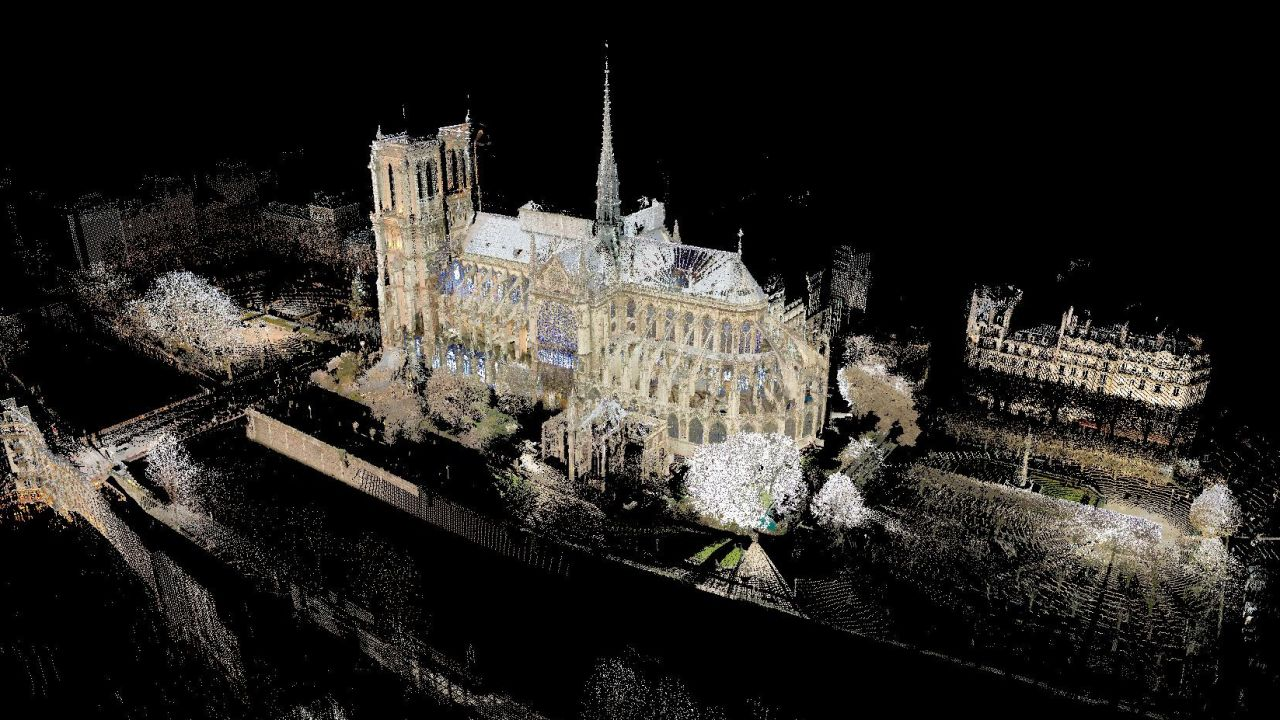
\includegraphics[width=0.84\linewidth]{figures/notre_dame_lidar_scan.png}
    \caption{اسکن رنگی لایدار از ساختمان معروف نوتردام پاریس که با استفاده از آن این ساختمان را بازسازی کردند.}
    \label{fig:notre_dame_lidar}
\end{figure}
فضایی واحد بر روی سطح شیء است. با تجمع این نقاط، ابر نقاط کل سطح خارجی یک شیء را می‌تواند نمایان کند. اگر مقادیر رنگ هر نقطه نیز اندازه‌گیری شود، اطلاعات رنگی نیز می‌تواند به ابر نقاط افزوده شود.
\begin{figure}[h]
    \centering
    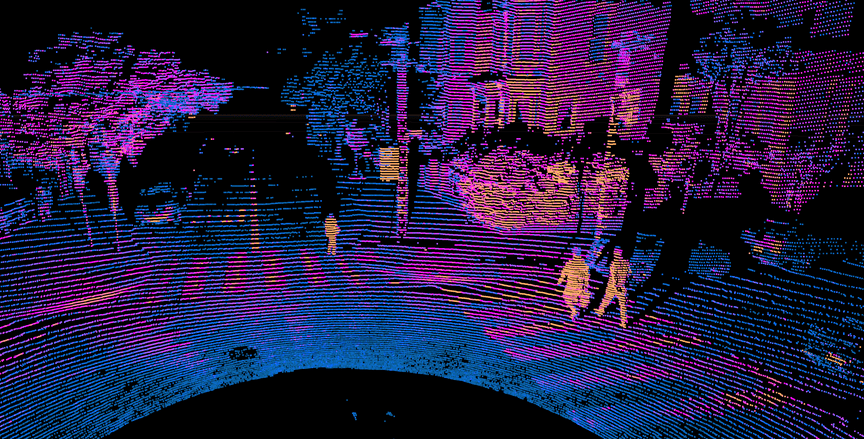
\includegraphics[width=0.84\linewidth]{vehicle_lidar_scan.png}
    \caption{اسکن لایدار \lr{OS1:64} از شرکت \lr{Ouster} که بر روی یک ماشین نصب شده است.}
    \label{fig:vehicle_lidar_scan}
\end{figure}
ابر نقاط با استفاده از یک اسکنر سه‌بعدی، لایدار یا نرم‌افزار فتوگرامتری\LTRfootnote{\lr{Photogrammetry}} ایجاد می‌شود.

در حوزه‌ی خودروهای خودران و سیستم‌های مدیریت هوشمند ترافیک نیز از لایدارها استفاده می‌شود تا ابر نقاط حاصل از فضای دور ماشین یا جاده‌ها به عنوان ورودی به مدل‌های هوش مصنوعی داده شود و اجسام داخل این فضا شناسایی شوند.

\subsubsection{تشخیص اجسام سه‌بعدی}
ادراک فضای سه‌بعدی یک پیش‌نیاز در حوزه رانندگی خودکار و دوقلوی دیجیتال است. درک کامل از آنچه که در حال حاضر در جلوی حسگر رخ می‌دهد، تسهیل‌دهنده‌ای برای اجزای پایین-دست\LTRfootnote{\lr{Downstream}} است تا به موقع واکنش نشان دهند. این همان چیزی است که تشخیص اجسام سه‌بعدی\LTRfootnote{\lr{3D Object Detection}} را هدف قرار می‌دهد.
\begin{figure}[h]
    \centering
    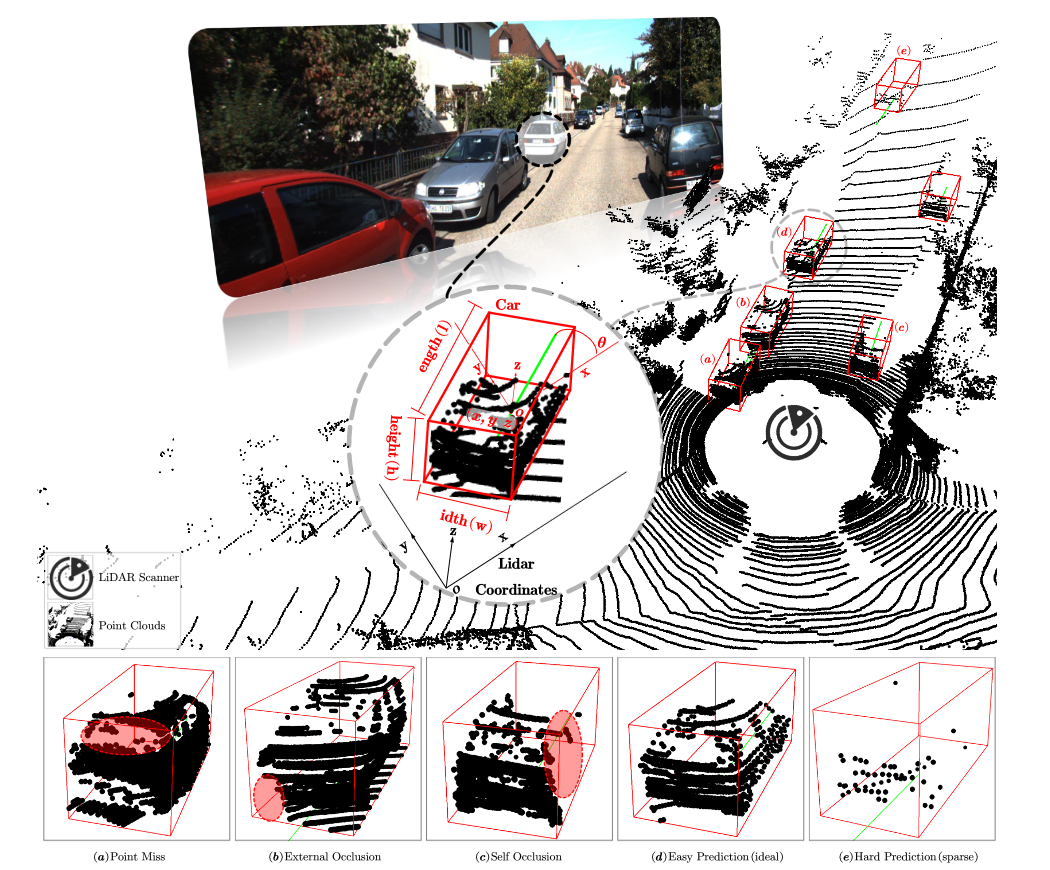
\includegraphics[width=1\linewidth]{figures/3D_Object_Detection_Overview.png}
    \caption{بررسی اجمالی وظیفه‌ی تشخیص اجسام سه‌بعدی از تصاویر و ابر نقاط\cite{qian20223d}}
    \label{fig:3d_object_detection_overview}
\end{figure}تشخیص اجسام سه‌بعدی، فضای اطراف ما را از طریق اختصاص یک برچسب\LTRfootnote{\lr{Label}}، تعیین شکل اجسام با کشیدن کادر محصورکننده\LTRfootnote{\lr{Bounding Box}}، و اعلام فاصله اجسام از حسگر توصیف می‌کند. علاوه بر این، تشخیص سه‌بعدی حتی زاویه‌ی جهت‌گیری\LTRfootnote{\lr{Orientation}} اجسام را به ما می‌دهد. این اطلاعات بدست‌ آمده از پشته‌ی ادراک\LTRfootnote{\lr{Detection Stack}}، این امکان را فراهم می‌کند که مدل‌های برنامه‌ریزی پایین-دست تصمیم‌گیری کنند \cite{qian20223d}.

\cref{fig:3d_object_detection_overview} یک بررسی اجمالی از تشخیص اجسام سه‌بعدی با استفاده از ابر نقاط و تصویر را نشان می‌دهد.
مشاهده می‌کنیم که چالش‌هایی در تشخیص اجسام سه‌بعدی داریم:
\begin{itemize}
    \item \lr{a}) عدم دریافت نقطه:‌ هنگامی که سیگنال‌های لایدار نتوانند از سطح شئ بازتاب شوند و به حسگر برگردند.
    \item \lr{b}) مسدودی از بیرون:‌ هنگامی که سیگنال‌های لایدار توسط موانع اطراف مسدود شوند.
    \item \lr{c}) مسدودی از درون: هنگامی که طرف نزدیک شئ طرف دیگر آنرا مسدود کند، که ابر نقطه جسم را در عمل به ابر نقطه‌ای ۵.۲ بعدی تبدیل می‌کند. 
\end{itemize}
مشاهده می‌کنیم که پیش‌بینی کادر محصورکننده‌ در مورد \lr{(d)} به مراتب آسان‌تر از مورد \lr{(e)} است؛ زیرا اجسامی که در فواصل دورتر از لایدار هستند، نقاط پراکنده و به اصطلاح تنک‌تری\LTRfootnote{\lr{Sparse}} دارند.

هدف اصلی تشخیص اجسام سه‌بعدی، تشخیص اجسام با ایجاد کادر محصور‌کننده سه‌بعدی و اختصاص برچسب به آنها است. برای حل این مسئله دو مدل متداول تشخیص اجسام سه‌بعدی، یعنی تصاویر و ابر نقاط، با چالش‌های مختلفی روبرو می‌شوند. با استفاده تنها از تصاویر، چالش اصلی عدم وجود اطلاعات عمق اجسام است؛ زیرا با وجود پیشرفت‌های زیاد در زمینه بازیابی عمق از تصاویر، این مسئله هنوز یک مسئله با پیچیدگی بالا و حل نشده محسوب می‌شود. همچنین، یک شئ در وضعیت‌های سه‌بعدی مختلف ممکن است به نمایش‌های تصویری مختلفی منجر شود، که برای یادگیری نمایش کادرها سودمند نیست. علاوه بر این، از آنجا که دوربین حسگری غیرفعال\LTRfootnote{\lr{Passive Sensor}} است، تصاویر طبیعتا نسبت به روشنایی (به عنوان مثال در شب) یا شرایط جوی (هوای بارانی) تاثیرپذیرند. از سوی دیگر، با استفاده تنها از ابر نقاط، مواجهه با چالش‌های مربوط به یادگیری بازنمایی\LTRfootnote{\lr{Representation Learning}} کادر محصورکننده‌ی اجسام رخ می‌دهد. طبیعت ابر نقاط، بی‌نظمی و تنک بودن است، به همین دلیل اعمال پیچش بر روی آن، منجر به "از دست رفتن اطلاعات شکل و واریانس در ترتیب نقاط" می‌شود. به علاوه، ابر نقاط در عمل دو و نیم‌بعدی هستند که مشکلات آن در \cref{fig:3d_object_detection_overview} قابل مشاهده است. با حذف المان استفاده از شبکه‌های عصبی پیچشی، یک راه برای نمایش ابر نقاط، نمایش آنها به عنوان شبکه‌ای از واکسل‌ها\LTRfootnote{\lr{Voxel Grid}} می‌باشد. معضل این روش این است که افزایش اندازه مکعب واکسل، باعث از دست دادن وضوح و به تبع آن کاهش دقت مکان‌یابی می‌شود؛ در حالی که کاهش اندازه آن، پیچیدگی و استفاده از حافظه را افزایش می‌دهد. راه دیگر نمایش ابر نقاط به عنوان مجموعه‌هایی از نقاط\LTRfootnote{\lr{Point Sets}} می‌باشد. با این حال، حدود 80 درصد زمان اجرا توسط بازیابی نقاط اشغال می‌شود که سرعت را به شدت کند می‌کند. با داشتن هم‌زمان هم تصاویر و هم ابر نقاط، مشکل دشوار اغلب اوقات مطابقت معنایی\LTRfootnote{\lr{Semantic Alignment}} بین تصویر و ابر نقاط است. تصاویر و ابر نقاط دو منبع داده غیرهمگن\LTRfootnote{\lr{Heterogeneous}} هستند که توسط زاویه دید دوربین و زاویه دید سه‌بعدی واقعی لایدار نمایش داده می‌شوند. نتیجه تطابق نقطه‌ای بین نقاط لایدار و پیکسل‌های تصویر منجر به \textbf{محو شدن ویژگی}\LTRfootnote{\lr{Feature Blurring}} می‌شود \cite{qian20223d}.

از آنجایی که در این پژوهش از دوربین برای تشخیص اجسام استفاده نشده است، به روش‌های تشخیص اجسام سه‌بعدی مبتنی بر ابر نقاط روی آورده شده است.

\subsubsection{روش‌های مبتنی بر ابر نقاط}

شبکه‌های عصبی پیچشی همواره به دلیل قابلیت بهره‌برداری از همبستگی‌های\LTRfootnote{\lr{Correlation}}  محلی در فضای همسایگی پیکسل‌های موجود در شبکه‌های منظم متراکم (مانند تصاویر)، در علم بینایی ماشین به کار گرفته‌ شده‌اند. اما نقاط داخل ابر نقاط به صورت پخش شده و تنک، با ساختاری نامنظم و بدون ترتیب می‌باشند. به عبارت دیگر، استفاده مستقیم از عملگر پیچش بر روی ابر نقاط، به اعوجاج بازنمایی آنها منجر خواهد شد. برای رفع مشکلات ذکرشده، برخی از مقالات ورودی‌های خود را به شکل واکسلی تجزیه و تحلیل می‌کنند تا با عملگر پیچش قابل تطبیق باشند، در حالی که کارهای دیگر به آخرین پیشرفت‌ها در زمینه یادگیری ویژگی‌ها و معنای بین نقاط در مجموعه نقاط، رجوع می‌کنند. بر اساس راه‌کارهای یادگیری بازنمایی ابر نقاط، این مطالعات به سه گروه زیر تقسیم می‌شوند:
\begin{enumerate}
    \item روش‌های مبتنی بر واکسل \LTRfootnote{\lr{Voxel Based Methods}}
    \item روش‌های مبتنی بر نقطه \LTRfootnote{\lr{Point Based Methods}}
    \item روش‌های مبتنی بر واکسل-نقطه\LTRfootnote{\lr{Voxel-Point Based Methods}}
\end{enumerate}

همانطور که در \cref{fig:evolution_point_cloude_based} مشاهده می‌کنیم، سیر تکامل روش‌های مختلف تشخیص مبتنی بر ابر نقاط قابل مشاهده هستند. روش‌های مبتنی بر نقطه و مبتنی بر واکسل-نقطه نسبتا جدید هستند و به نظر می‌آید که در آینده مدل‌های بیشتری را در این گروه‌ها مشاهده خواهیم کرد \cite{qian20223d}.

\begin{figure}[h]
    \centering
    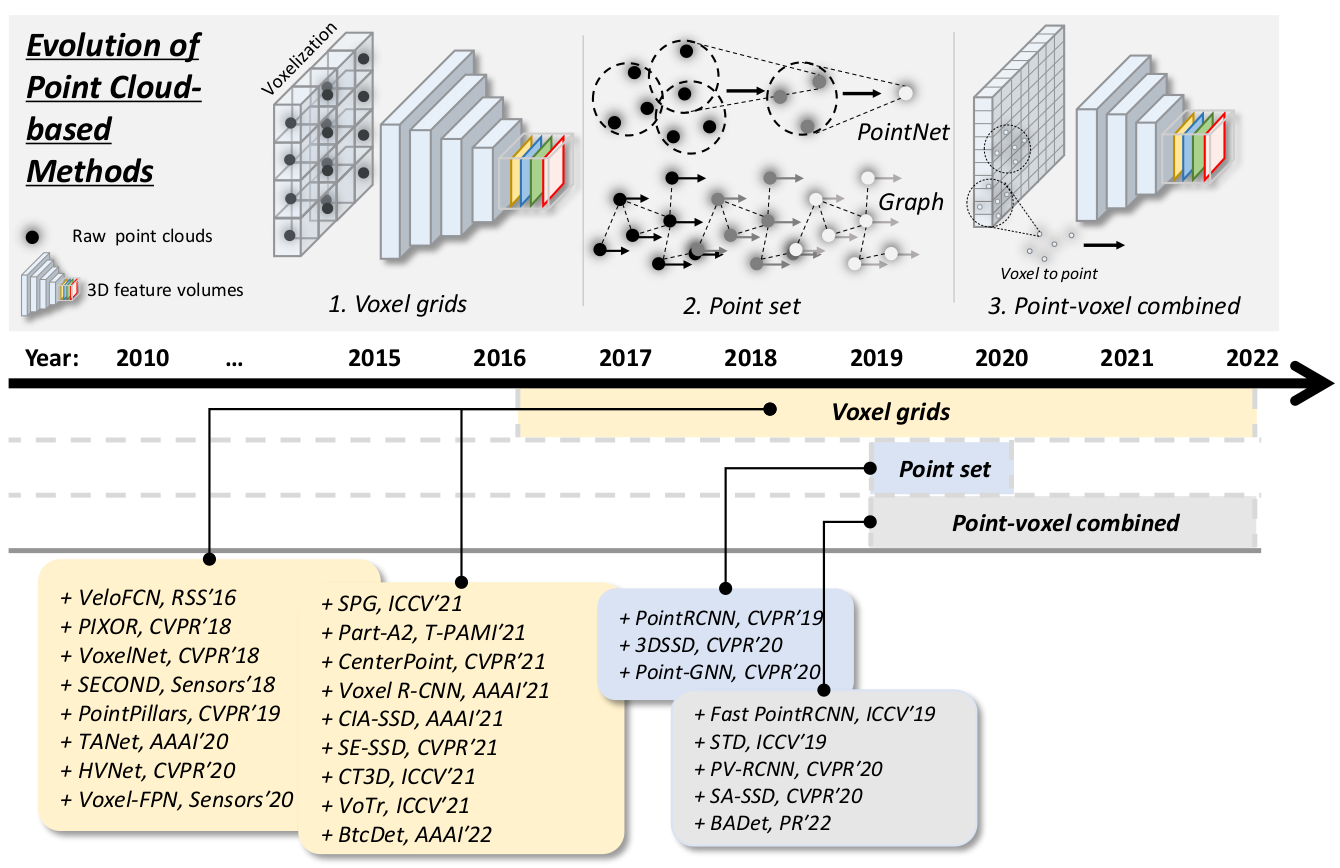
\includegraphics[width=1\linewidth]{figures/evolution_point_cloud_based.png}
    \caption{سیر زمانی پیشرفت روش‌های مبتنی بر ابر نقاط \cite{qian20223d}}
    \label{fig:evolution_point_cloude_based}
\end{figure}

\subsubsection{روش‌های تشخیص مبتنی بر واکسل}

این گروه از روش‌ها، ابر نقاط نامنظم را به شبکه‌های مرتب و فشرده دو بعدی و سه بعدی تبدیل می‌کنند. سپس آن‌ها را به شکل نمای دید پرنده\LTRfootnote{\lr{Bird's Eye View (BEV)}} دو بعدی تبدیل می‌کنند تا شبکه‌های پیچشی همانند تصاویر با آن برخورد کنند و توابع پیچش موثر و سریع‌تری داشته باشند. به عنوان مثال، مدل \lr{VoxelNet} ابر نقاط را به شبکه‌های واکسلی متراکم تقسیم‌بندی می‌کند و از شبکه‌های عصبی پیچشی سه بعدی برای پیچش در امتداد هر بعد استفاده می‌کند، اگرچه این رویکرد با هزینه محاسباتی و حافظه زیادی همراه است. از سوی دیگر، مدل \lr{SECOND} از عملیات پیچش پراکنده\LTRfootnote{\lr{Sparse Convolution}} استفاده می‌کند تا محاسبات غیرضروری ناشی از لایه‌گذاری صفر\LTRfootnote{\lr{Zero Padding}} در واکسل‌ها را کاهش دهد. مدلی معروف به نام \lr{PointPillars} واکسل‌ها را به شکل ستون‌های دربرگیرنده کل نقاط در راستای عمودی، در نمای دید پرنده امتداد می‌دهد. البته این روش به قیمت کاهش وضوح عمودی تمام می‌شود که بر کیفیت یادگیری بازنمایی تاثیر می‌گذارد، اما سرعت چشم‌گیری دارد \cite{qian20223d}.

برای مهار کردن این محدودیت \lr{PointPillars}، برخی از روش‌ها به شبکه‌های واکسلی باز‌گشتند. مدل \lr{Voxel R-CNN} ویژگی‌های واکسلی را با استفاده از پیچش‌های سه‌بعدی برای بهبود پیشنهاد\LTRfootnote{\lr{Proposal Refinement}}، جمع‌آوری می‌کند، در حالی که مدل \lr{SE-SSD} هم‌زمان یک شبکه عصبی دانش‌آموز را تحت راهنمایی دانش تصفیه‌شده شبکه عصبی استاد، نظارت می‌کند. روش‌های دیگر، استراتژی‌های چندمقیاسه واکسلیزه کردن را به جمع‌آوری ویژگی\LTRfootnote{\lr{Feature Extraction}} اضافه می‌کنند، از وابستگی‌های زمینه‌ای بین واکسل‌هایی با فواصل زیاد\LTRfootnote{\lr{Long Range Contextual Dependancies}} بهره‌می‌برند یا یادگیری شکل\LTRfootnote{\lr{Shape Learning}} را برای مقابله با مسائل مربوط به کیفیت ابر نقاط تحت تأثیر عواملی مانند شرایط جوی نامساعد، انسداد\LTRfootnote{\lr{Occlusion}} و انتهای افق دید لایدار به کار می‌گیرند. لازم به ذکر است که روش‌های مبتنی بر شبکه‌های واکسلی، از بازنمایی نمای دید پرنده مرتبط بهره‌می‌برند که ابهام در مقیاس را کاهش می‌دهد و حداقل انسدادها را دارد \cite{qian20223d}.

\subsubsection{روش‌های تشخیص مبتنی بر نقطه}
این دسته از روش‌ها از عامل‌هایی استفاده می‌کنند که وابسته به ترتیب نیستند و در نتیجه امکان شناسایی ساختارهای محلی و الگوهای پیچیده در ابر نقاط را بدون نیاز به کوانتش\LTRfootnote{\lr{Quantization}} ممکن می‌سازند. این رویکرد، خصوصیات هندسی و ذاتی ابر نقاط خام را حفظ می‌کند. به عنوان مثال، مدل \lr{PointRCNN} از یک تکنیک مشابه مدل معروف \lr{PointNet} برای یادگیری نشانه‌های معنادار\LTRfootnote{\lr{Semantic Cues}} نقاط گوشه‌ای جسم تشخیص داده شده استفاده می‌کند، که امکان تولید پیشنهادات سه‌بعدی\LTRfootnote{\lr{3D Proposals}} برای شکل جسم را به صورت گام‌به‌گام ممکن می‌سازد. لازم به ذکر است که روش‌های مجموعه‌ی \lr{PointNet}، به طور گسترده‌ای از ابزارهای نمونه‌افزایی\LTRfootnote{\lr{Upsampling}} و پخش اطلاعات مفهومی در نقاط کلیدی بهره می‌برند.

از طرف دیگر، رویکرد مدل \lr{3DSSD} برای افزایش بهره‌وری سیاست نمونه‌برداری نقاط، نگرشی تازه به فاصله ویژگی‌های\LTRfootnote{Feature Distance} نقاط به همراه فاصله اقلیدسی\LTRfootnote{Euclidean Distance} آن‌ها می‌اندازد. مدل \lr{Point-GNN} با الهام گرفتن از عملکرد موفق ابر نقاط در وظایفی مانند طبقه‌بندی\LTRfootnote{Classification} و بخش‌بندی معنایی\LTRfootnote{Semantic Segmentation}، تصمیم‌گیری را بر اساس گراف‌های همسایه محلی نقاط ساخته شده‌اند، انجام می‌دهد. در این گراف‌ها، هر گره به صورت تدریجی اطلاعات مفهومی را از نواحی مجاور خود جمع‌آوری می‌کند. با این حال، لازم به ذکر است که روش‌های مبتنی بر نقاط، ممکن است مصرف محاسباتی بسیار بالایی داشته باشند و با پیچیدگی جستجوی توپی\LTRfootnote{‌Ball Query Complexity} \lr{O(k$\cdot$|$\chi$|)} مواجه باشند. برخی رویکردها این چالش را با پیاده‌سازی گروه‌بندی چند مقیاسی و چند رزولوشنی حل می‌کنند؛ اما این روش با افزایش تعداد نقاط در مجموعه \lr{$\chi$}، سربار پردازشی خواهد داشت \cite{qian20223d}.

\subsubsection{روش‌های تشخیص مبتنی بر واکسل-نقطه}

روش‌های موجود در این دسته، یک رویکرد نوآورانه معرفی می‌کنند که نقاط قوت دو روش قبلی را ترکیب می‌کند. روش‌های مبتنی بر واکسل از لحاظ محاسباتی کارآمد هستند، اما ممکن است الگوهای ریز همانند انسان‌ها را نادیده بگیرند و بر روی بهبود دقت در هر تکرار\LTRfootnote{\lr{Iteration}} یادگیری، تاثیر منفی بگذارند. متقابلا، روش‌های مبتنی بر نقاط معمولاً تاخیر نسبی بیشتری دارند اما در حفظ ناهنجاری و محلی بودن ابر نقاط بهتر عمل می‌کنند. به عنوان مثال، مدل \lr{STD} از \lr{PointNet++} برای متراکم‌سازی اطلاعات معنادار بین نقاط پراکنده استفاده می‌کند، سپس آنها را واکسلیزه  می‌‌کند و یک بازنمایی متراکم‌تر برای بهبود دقت ایجاد می‌کند.  مدل \lr{PV-RCNN}، با یکپارچه‌کردن بهره‌وری اطلاعات مفید با استفاده از عملیات پیچش پراکنده سه‌بعدی\LTRfootnote{\lr{3D Sparse Convolutions}}، و استخراج داده‌های حائز اهمیت و معنادار با استفاده از مجموعه‌های شبه  \lr{PointNet}، فرآیند یادگیری معانی متمایزتر را تقویت می‌کند. مدل \lr{SA-SSD}، با استفاده از یک شبکه عصبی کمکی، ویژگی‌های واکسل‌هایی که با استفاده از پیچش پراکنده سه‌بعدی بدست آمده است را نسبت به ساختار نقاط خود آگاه‌تر می‌کند. یعنی این شبکه عصبی کمکی، ساختار اشکال داخل واکسل‌ها را حدس می‌زند و سعی می‌کند اشکالی که نقاط آنها ناقص هستند را تکمیل کند \cite{qian20223d}.

\subsubsection{تشخیص اجسام سه‌بعدی در دوقلوهای دیجیتال}

در حال حاضر، به نظر می‌آید که روش‌های مبتنی بر واکسل انتخاب اصلی محققین هستند، همانطور که در \cref{fig:evolution_point_cloude_based} نیز مشاهده می‌شود. روش‌های مبتنی بر واکسل، قابلیت انعطاف بالا برای پیاده‌سازی در سخت‌افزار را دارند و دقتی قابل توجه و زمان پاسخ نسبتاً کمتری دارند. از سوی دیگر، روش‌های مبتنی بر نقطه توانایی حفظ ویژگی‌های محلی فضایی\LTRfootnote{\lr{Spatially-Local Features}} ابرنقاط را دارند، اما نسبت به روش‌های مبتنی بر واکسل زمان بیشتری برای پیشروی رو به جلو\LTRfootnote{\lr{Feedforward}} دارند. با مقایسه سه روش تشخیص مبتنی بر ابر نقاط، آشکار می‌شود که روش‌های مبتنی بر واکسل، همچنان به عنوان جهتی بسیار امیدبخش‌تر در کاربردهای بلادرنگ، به عنوان مثال در حوزه رانندگی خودروهای خودران و دوقلوهای دیجیتال، مورد مطالعه قرار گرفته شده‌اند.

\subsection{مجموعه داده مدل‌های تشخیص سه‌بعدی}

دسترسی به مجموعه‌ داده‌هایی\LTRfootnote{\lr{Datasets}} با مقیاس‌های عظیم، نقش مهمی در پیشرفت حوزه‌های مختلف هوش‌ مصنوعی ایفا کرده است. در زمینه تشخیص اجسام سه‌بعدی، چندین مجموعه داده عمومی به تحقیقات کمک کرده‌اند. مجموعه‌ داده‌های معروفی از جمله \lr{KITTI} \cite{geiger2012we}، \lr{nuScenes} \cite{caesar2020nuscenes}، و \lr{Waymo Open} \cite{sun2020scalability}   وجود دارند که به عنوان  منابع گسترده برای کاربردهای مرتبط با خودرو‌های خودران به کار می‌روند. این مجموعه‌ داده‌ها در ابعاد مختلف از جمله اندازه\LTRfootnote{\lr{Size}}، تنوع\LTRfootnote{\lr{Diversity}}، مزایا و معایب با یکدیگر تفاوت دارند.

\subsubsection{اندازه}

مجموعه داده \lr{KITTI} شامل 200,000 کادر محصورکننده حاشیه‌نویسی شده\LTRfootnote{\lr{Annotated Bounding Boxes}} و توزیع شده در 15,000 فریم می‌شود. این مجموعه داده برای آموزش و آزمون، نمونه‌هایی تقریباً مشابه دارد. در مقابل، مجموعه داده \lr{nuScenes} شامل 1.4 میلیون کادر محصورکننده توزیع شده در 40,000 فریم است و مجموعه‌هایی جدا و متمایز برای آموزش، اعتبارسنجی و آزمون دارد. مجموعه داده \lr{Waymo Open} با بیش از 112 میلیون کادر محصورکننده در 200,000 فریم و داده‌هایی با مقیاس بزرگ برای آموزش، اعتبارسنجی و آزمون، از سایرین برجسته‌تر است. لازم به ذکر است که در حالی که حاشیه‌نویسی‌ها برای آموزش و اعتبارسنجی در دسترس هستند، هیچ یک از این مجموعه‌های داده حاشیه‌نویسی‌ای برای مجموعه‌ آزمون ارائه نمی‌دهند و شرکت‌کنندگان باید پیش‌بینی‌های خود را در وبسایت آنلاین مجموعه‌ داده‌ها  ارسال کرده و ارزیابی\LTRfootnote{\lr{Benchmark}} کنند \cite{qian20223d}.

\subsubsection{تنوع}

مجموعه داده \lr{KITTI}، داده‌ها را از 50 صحنه ترافیکی مختلف با 8 کلاس اجسام فراهم می‌کند و ارزیابی آنلاین آن بر روی کلاس‌های خودرو، پیاده‌رو و دوچرخه‌سوار تمرکز دارد. این مجموعه داده صحنه‌ها را بر اساس میزان ارتفاع کادر‌های محصور کننده دوبعدی، میزان انسداد در ابرنقاط و میزان برش ابرنقاط به علت رسیدن به انتهای افق دید لایدار، طبقه‌بندی می‌کند. از طرفی، مجموعه داده \lr{nuScenes} از 1,000 صحنه ترافیکی در 23 کلاس داده ارائه می‌دهد و در ارزیابی آنلاین، تمرکز خود را بر روی 10 کلاس تشخیص اجسام سه‌بعدی می‌گذارد. مجموعه داده \lr{Waymo Open} شامل 1,150 صحنه ترافیکی در 4 کلاس است و ارزیابی آنلاین آن بر روی سه کلاس مشابه با \lr{KITTI} تمرکز دارد. لازم به ذکر است که مجموعه داده‌های \lr{nuScenes} و \lr{Waymo Open}، داده‌های خود را در شرایط جوی و روشنایی مختلف شامل باران، مه، برف، روز و شب جمع‌آوری کرده‌اند و تنوع بیشتری در سناریوها نسبت به \lr{KITTI} ارائه می‌دهند، که تنها به روزهای آفتابی محدود است \cite{qian20223d}.

\begin{table}[h!]
    \centering
    \caption{توزیع داده در داده‌های آموزش \lr{KITTI}. کلاس خودرو \% 99.82 سه کلاس اصلی (خودرو، عابرپیاده، دوچرخه‌سوار) را تشکیل می‌دهد \cite{qian20223d}.}
    \begin{tabular}{ccccccccc}
         \hline
         کلاس & انسان نشسته & قطار & غیره & کامیون & دوچرخه‌سوار & ون & عابر‌پیاده & خودرو  \\
         \hline
          تعداد & 56 & 224 & 337 & 448 & 734 & 1297 & 2,207 & 14,357 \\
         \hline
    \end{tabular}
    \label{tab:KITTI_class_table}
\end{table}

\begin{table}[h!]
    \centering
    \caption{توزیع داده در داده‌های آموزش \lr{nuScenes} \cite{qian20223d}.}
    \label{tab:nuSceness_class_table}
    \begin{tabular}{ccccccccc}
         \hline
         کلاس & اتوبوس & تریلی & کامیون & مخروط ترافیکی & مانع ترافیکی & عابر پیاده & خودرو\\
         \hline
         تعداد & 13,163 & 20,701 & 72,815 & 82,362 & 125,095 & 185,847 & 413,318 \\
         \hline
    \end{tabular}
    
    \begin{tabular}{cccc}
        \\
        \hline
        کلاس‌ & دوچرخه & موتورسیکلت & جرثقیل \\
        \hline
         تعداد & 9,478 & 10,109 & 11,993 \\
        \hline
    \end{tabular}
\end{table}

\subsubsection{مزایا و معایب}

این مجموعه‌ داده‌ها تاثیر قابل توجهی بر جامعه علمی داشته‌اند. به ویژه \lr{KITTI} تأثیر عمیقی در زمینه‌های جمع‌آوری داده‌ها، پروتکل‌ها و ارزیابی‌ داشته است. با این حال، بایستی توجه داشت که جمع‌آوری داده‌های \lr{KITTI}، تنها در روزهای آفتابی انجام شده است. یعنی شرایط روشنایی و جوی که می‌تواند تأثیر زیادی بر سناریوهای واقعی داشته باشد، در نظر گرفته نشده است. این مشکل توسط مجموعه داده‌های \lr{nuScenes} و \lr{Waymo Open} حل شده است. این دو مجموعه‌ داده، داده‌های خود را در شرایط مختلف جوی و روشنایی مانند باران، مه، برف، روز و شب جمع‌آوری می‌کنند. علاوه بر این، مجموعه‌ داده‌های واقعی معمولاً از عدم توازن کلاس‌ها\LTRfootnote{\lr{Data Imbalance}} رنج می‌برند، که اکثر کلاس‌های آنها به درصد کوچکی از دسته‌ها تعلق دارند. با توجه به \cref{tab:KITTI_class_table} و \cref{tab:nuSceness_class_table}، می‌توان این مشکل را در مجموعه‌ داده‌های \lr{nuScenes} و \lr{KITTI} مشاهده کرد \cite{qian20223d}. 

\subsection{معیارهای ارزیابی}

در بخش قبلی مشاهده کردیم که مجموعه دادگانی وجود دارند که برای آموزش، آزمون و ارزیابی مدل‌های تشخیص اجسام سه‌بعدی،‌ طراحی شده‌اند. حال به روش‌هایی که این مجموعه‌دادگان با استفاده از آن مدل را ارزیابی می‌کنند، می‌پردازیم. در ابتدا لازم است که مفاهیمی را توضیح دهیم:

\subsubsection{ماتریس درهم‌ ریختگی}

 ماتریس درهم‌ ریختگی\LTRfootnote{\lr{Confusion Matrix}}، ابزاری حیاتی در یادگیری ماشین و آمار است. \begin{figure}[h!]
    \centering
    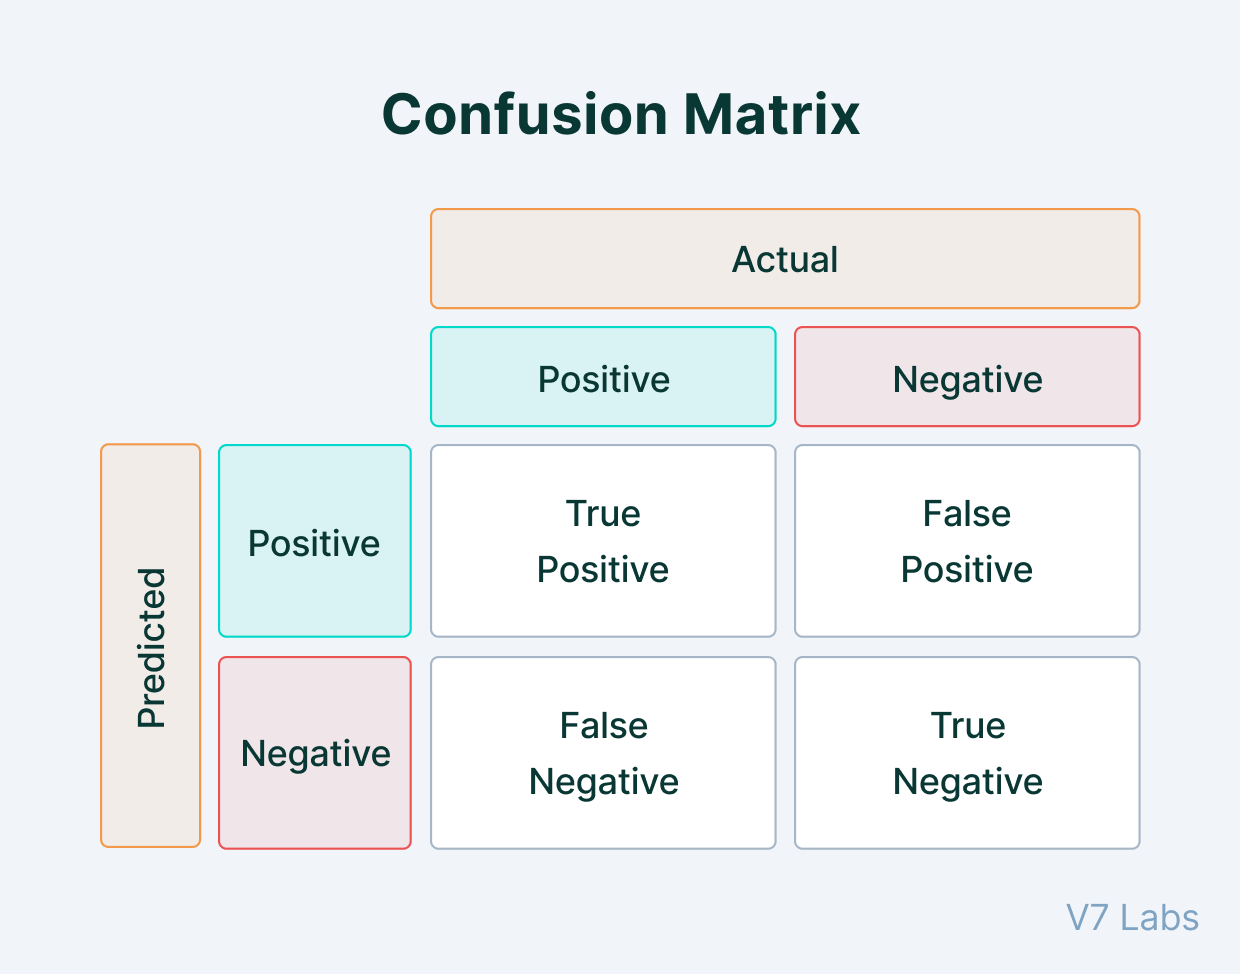
\includegraphics[width=0.75\linewidth]{figures/Confusion_Matrix.png}
    \caption{ماتریس در هم‌ ریختگی \cite{V7:mAP_Explanation}}
    \label{fig:confusion_matrix}
\end{figure}این ماتریس، خلاصه‌ای از مقایسه‌ پیش‌بینی‌های مدل با مقادیر واقعی\LTRfootnote{\lr{Ground Truth}} ارائه می‌دهد. این ماتریس از چهار بخش تشکیل شده است:
 \begin{enumerate}
     \item مثبت‌های واقعی\LTRfootnote{\lr{True Positive (TP)}} (نمونه‌های مثبتی که به درستی تشخیص داده شده‌اند)
     \item منفی‌های واقعی\LTRfootnote{\lr{True Negative (TN)}} (نمونه‌های منفی که درستی تشخیص داده شده‌اند)
     \item مثبت‌های کاذب\LTRfootnote{\lr{False Positives (FP)}} (نمونه‌های منفی‌ که به اشتباه به عنوان مثبت تشخیص داده شده‌اند)
     \item منفی‌های کاذب\LTRfootnote{\lr{False Negatives (FN)}} (نمونه‌های مثبت که به اشتباه به عنوان منفی تشخیص داده شده‌اند)
 \end{enumerate}

\subsubsection{دقت}
دقت\LTRfootnote{\lr{Precision}}، نشان‌دهنده این است که چه تعداد از نمونه‌هایی که مثبت پیش‌بینی شده‌اند، درست پیش‌بینی شده‌اند و رابطه‌ی آن از روش زیر قابل محاسبه است:
\begin{equation}
    Precision = \dfrac{TP}{TP+FP}
\end{equation}

\subsubsection{پوشش}
پوشش\LTRfootnote{\lr{Recall}}، مشخص می‌کند که چه تعداد از نمونه‌هایی که مثبت بوده‌اند، درست پیش‌بینی شده‌اند. رابطه‌ی آن به شکل زیر نوشته می‌شود:
\begin{equation}
    Recall = \dfrac{TP}{TP+FN}
\end{equation}

\subsubsection{نسبت اشتراک بر روی اجتماع}
معیار نسبت اشتراک بر روی اجتماع\LTRfootnote{\lr{Intersection over Union (IoU)}}، نشان‌دهنده انطباق مختصات کادر محصورکننده تخمین زده شده با کادر واقعی (یا داده‌های واقعی) است.

\begin{figure}[h!]
    \centering
    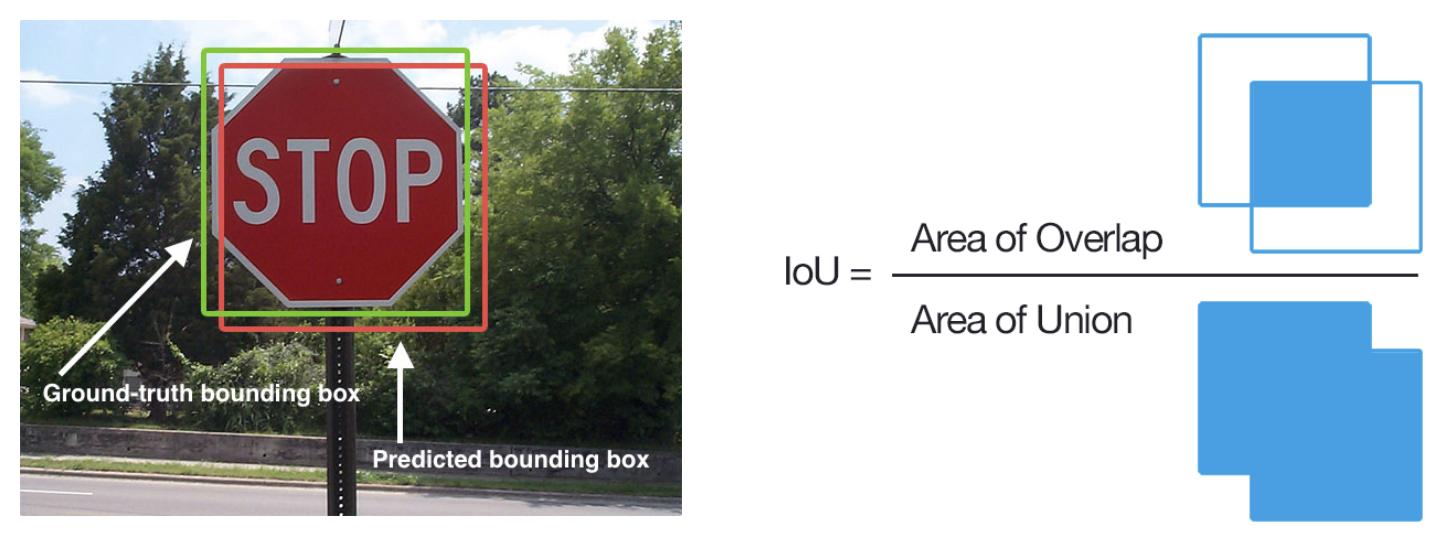
\includegraphics[width=0.8\linewidth]{figures/IoU.png}
    \caption{نسبت اشتراک بر روی اجتماع \cite{V7:mAP_Explanation}}
    \label{fig:IoU}
\end{figure}

همانطور که در \cref{fig:IoU} مشاهده می‌کنیم، نحوه محاسبه معیار نسبت اشتراک بر روی اجتماع نشان داده شده است. هدف از این کار، سنجیدن واقعی یا کاذب بودن تشخیص مدل است.

برای سنجش واقعی یا کاذب بودن، عموما حد آستانه‌ای\LTRfootnote{\lr{Threshold}} را برای نسبت اشتراک بر روی اجتماع می‌گذارند. به طور مثال در \cref{fig:IoU_FP_TP}، حد آستانه برابر با ۵.۰ است. پس کادر تخمینی‌ای که نسبت اشتراک بر روی اجتماع آن کمتر از این مقدار باشد، مثبت کاذب است و اگر بیشتر از حد آستانه باشد، مثبت واقعی است.

\begin{figure}[h!]
    \centering
    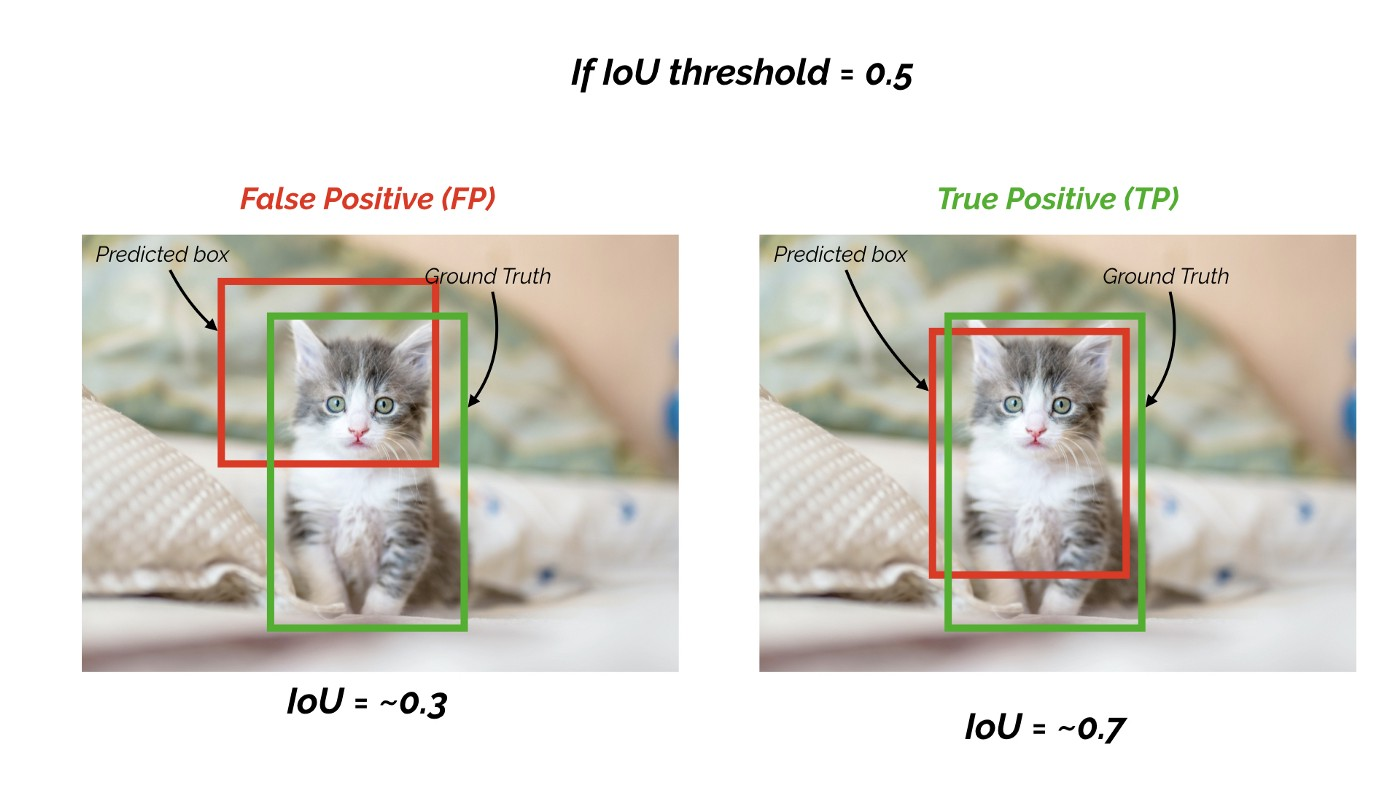
\includegraphics[width=0.8\linewidth]{figures/IoU_FP_TP.png}
    \caption{سنجش واقعی یا کاذب بودن براساس حد آستانه \cite{V7:mAP_Explanation}}
    \label{fig:IoU_FP_TP}
\end{figure}

\begin{figure}[h!]
    \centering
    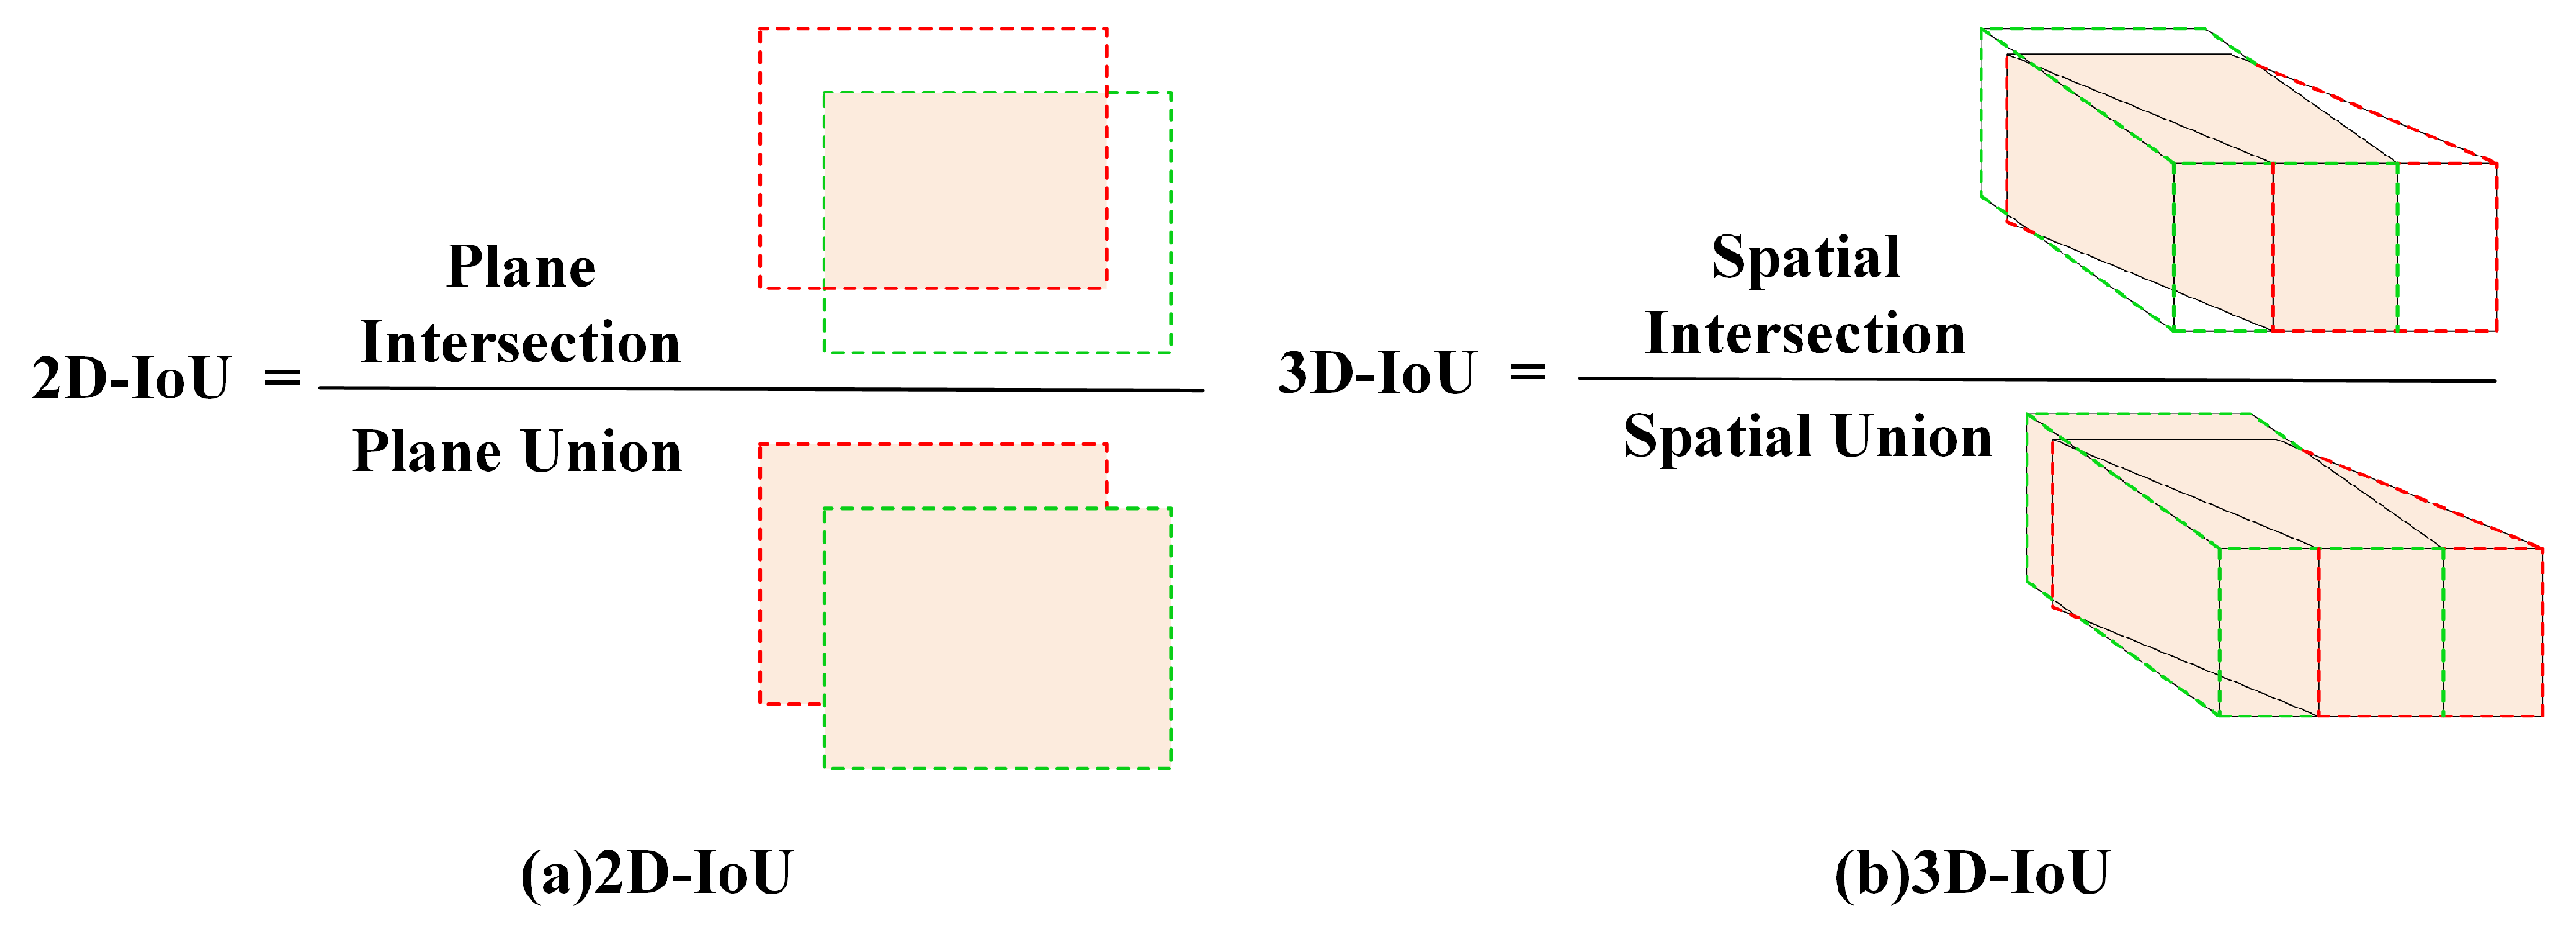
\includegraphics[width=0.8\linewidth]{figures/3d_IoU.png}
    \caption{نسبت اشتراک بر روی اجتماع در فضای سه‌بعدی و  دو بعدی \cite{han2022hybrid}}
    \label{fig:3d_IoU}
\end{figure}

این معیار فقط برای تصاویر دوبعدی نیست و در تشخیص اجسام سه‌بعدی نیز استفاده می‌شود. اما محاسبات این نسبت در اشکال سه‌بعدی بسیار دشوارتر است و عموما از تخمین برای محاسبه حجم مشترک استفاده می‌شود\LTRfootnote{\url{https://pytorch3d.org/docs/iou3d}}.


\subsubsection{میانگین دقت و میانگین دقت درون‌یابی شده}

در تشخیص اجسام سه‌بعدی و دوبعدی، امتیاز اطمینان\LTRfootnote{\lr{Confidence Score}} برای هر کادر محصورکننده تخمین زده شده محاسبه می‌شود. فرض کنیم زیرمجموعه نزولی پیش‌بینی‌‌ $\{y_1, \ldots, y_n\}$ وجود دارد که به ترتیب امتیاز اطمینان $s_i$ مرتب شده است؛ پیش‌بینی $y_i$ مثبت واقعی است اگر نسبت اشتراک بر روی اجتماع کادر محصورکننده $\beta_i$، از حد آستانه مشخص شده بیشتر باشد. اگر خلاف این باشد، مثبت کاذب است \cite{qian20223d}. نمودار زیگ-زاگی دقت-پوشش این زیرمجموعه، به راحتی قابل رسم است و مقدار میانگین دقت\LTRfootnote{\lr{Average Precision (AP)}} آن برابر با مساحت زیر نمودار است. اما در عمل، محاسبه‌ی مساحت زیر نمودار دشوار است. به همین دلیل محققانی در مسابقه \lr{PASCAL VOC}، روش‌هایی برای تسهیل محسابه میانگین دقت کشف کردند که از میانگین دقت درون‌یابی شده\LTRfootnote{\lr{Interpolated AP}} استفاده می‌کند.

برای درک بهتر محاسبه میانگین دقت درون‌یابی شده، مثالی آورده شده است. فرض کنیم تشخیص‌‌ دهنده اجسام، خروجی زیر را داده است و آن را براساس امتیاز اطمینان هر تصویر، مرتب کرده‌ است.

\begin{figure}[h!]
    \centering
    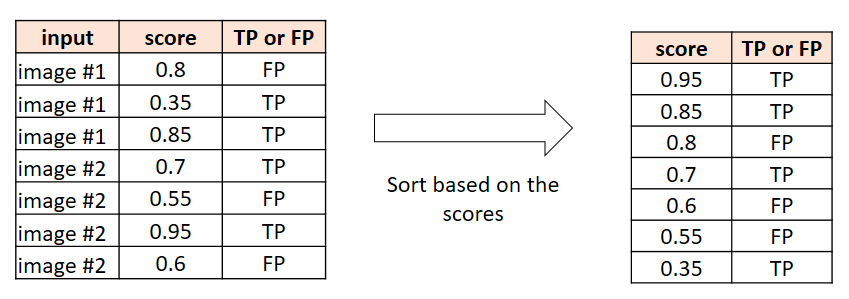
\includegraphics[width=1\linewidth]{figures/bbox_sorting.png}
    \caption{مرتب‌ سازی براساس امتیاز اطمینان کادرهای پیش‌بینی شده}
    \label{fig:bbox_sorting}
\end{figure}
حال مقادیر دقت و پوشش هر تخمین را به صورت تجمعی\LTRfootnote{\lr{Accumulated}} محاسبه می‌کنیم:

\begin{figure}[h!]
    \centering
    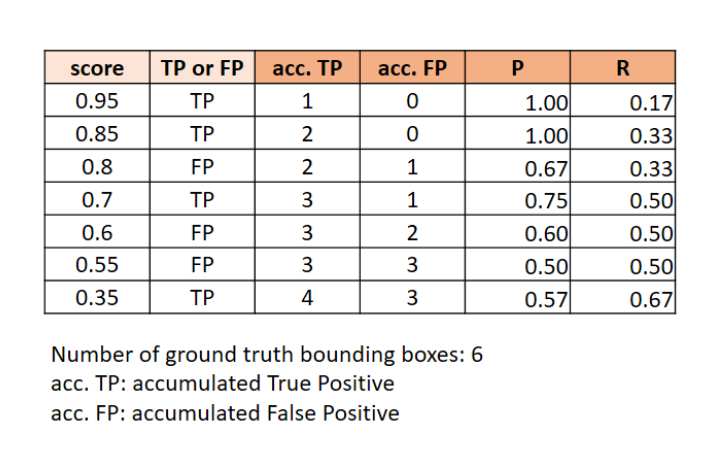
\includegraphics[width=0.75\linewidth]{figures/precision_recall_calculation.png}
    \caption{جدول محاسبه دقت و پوشش هر تخمین به صورت تجمعی}
    \label{fig:precision_recall_calculation}
\end{figure}

فرمول محاسبه پوشش و دقت به شکل زیر تعریف می‌شود:
\begin{equation}
    P = \dfrac{acc.TP}{acc.TP + acc.FP}\\
    R = \dfrac{acc.TP}{N}
    \label{P_R}
\end{equation}
که \lr{N} تعداد کادر محصورکننده‌های واقعی\LTRfootnote{\lr{Ground-Truth Bounding Boxes}} است. \cref{fig:precision_recall_calculation} جدول پوشش و دقت را نشان می‌دهد که با استفاده از \cref{P_R} محاسبه شده‌اند.
\\
\\
حال نمودار دقت-پوشش را رسم می‌کنیم. مشاهده می‌کنیم که نمودار به شکل زیگ-زاگی در آمده است. این اتفاق به علت مرتب‌سازی جدول براساس امتیاز اطمینان رخ داده است.

\begin{figure}[h!]
    \centering
    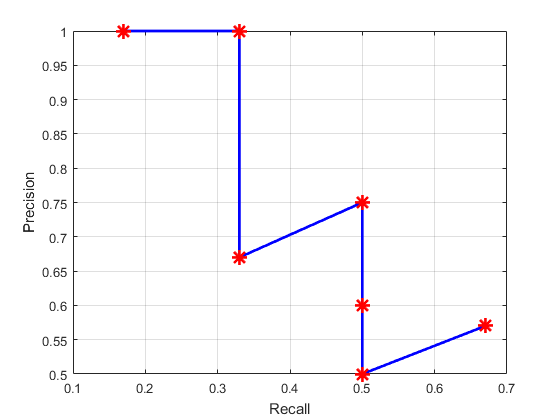
\includegraphics[width=0.8\linewidth]{figures/precision-recall_plot.png}
    \caption{نمودار دقت-پوشش}
    \label{fig:enter-label}
\end{figure}

برگزارکنندگان مسابقه \lr{PASCAL VOC} به دنبال راهی بودند که مساحت زیر نمودار دقت-پوشش را بتوان محاسبه کرد. از این رو به روش درون‌یابی میانگین دقت روی آوردند. 
\begin{definition}
    معیار پوشش درون‌یابی شده $AP \vert_{R_N}$، در زیرمجموعه پوشش $R$ محاسبه شده است که از $N$  سطح پوشش به شکل زیر تشکیل شده است \cite{qian20223d}: 
    \begin{equation}
        AP\vert_{R_N} = \frac{1}{N}\sum_{r\in{R}}{P_{interpolate}(r)}
        \label{AP_interpolate}
    \end{equation}
    که $R = \left[r_0, r_0 + \frac{r_1 - r_0}{N - 1}, r_0 + \frac{2(r_1 - r_0)}{N - 1}, \ldots, r_1\right]$. به ازای هر سطح پوشش $r$، دقت متناظر آن با بیشینه سطح پوشش‌های بیشتر یا مساوی $r$ درون‌یابی می‌شود، یا به عبارتی
    \begin{equation}
        P_{interpolate}(r) = \max_{\Tilde{r}:\Tilde{r}\ge r}{P(\Tilde{r})}
    \end{equation}
\end{definition}
حاصل درون‌یابی مثال زده شده، نمودار زیر است:
\begin{figure}[h!]
    \centering
    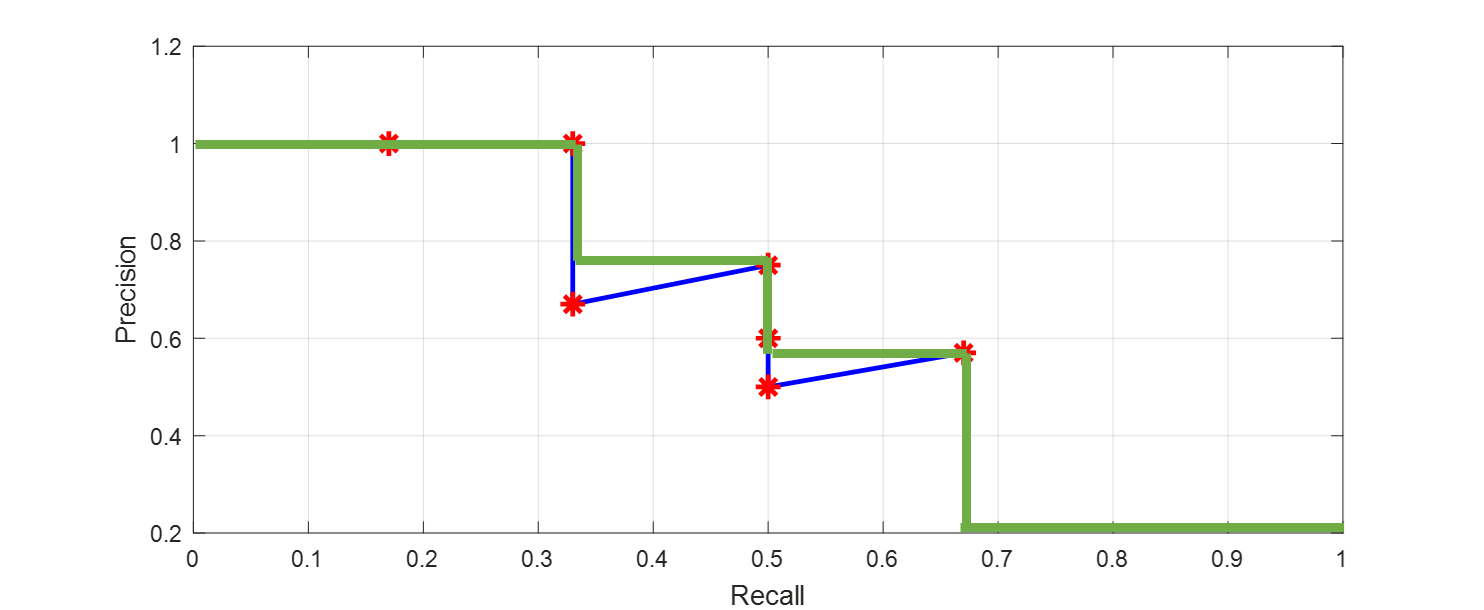
\includegraphics[width=1\linewidth]{figures/precision_recall_interpolate.png}
    \caption{نمودار دقت-پوشش درون‌یابی شده}
    \label{fig:precision-recall_interpolate}
\end{figure}

حال با فرض اینکه ۱۱ سطح پوشش داریم (طبق قرارداد \lr{PASCAL VOC} که البته در حال حاضر به ۴۰ سطح رسیده است)، میانگین دقت را طبق \cref{AP_interpolate}
 محاسبه می‌کنیم که خواهیم داشت:
 \begin{equation}
    AP = \frac{1}{11}(P_{interp}(0) + P_{interp}(0.1) + \ldots + P_{interp}(0.9) + P_{interp}(1))
 \end{equation}
 
\subsubsection{معیار \lr{mAP}}

معیار \lr{mAP}، عموما برای ارزیابی مدل‌های تشخیص اجسام در تصاویر دوبعدی (مانند \lr{Fast R-CNN}، \lr{YOLO}، \lr{Mask R-CNN} و غیره) استفاده می‌شود. این مقدار با میانگین گرفتن از میانگین دقت\LTRfootnote{\lr{Average Precision}} کلاس‌ها محاسبه می‌شود و مقداری بین ۰ تا ۱ دارد.

فرمول محاسبه‌ $mAP$ به شکل زیر است:
\begin{equation}
    mAP = \frac{1}{K}\sum_{C_i \in C}{AP_{Cـi}}
\end{equation}
 که $AP$ همان میانگین دقت است، $C$ مجموعه کلاس‌ها است و $K$ تعداد کلاس‌ها است. مقدار میانگین دقت می‌تواند به طور عادی با بدست آوردن سطح زیر نمودار محاسبه شود یا از حالت درون‌یابی شده آن یا $AP_{interpolate}$ استفاده شود. عموما از حالت دوم استفاده می‌شود زیرا نسبت به تغییرات پوشش حساس نیست و نتیجه بهتری می‌دهد.

 \subsubsection{معیار ارزیابی \lr{KITTI}}
مجموعه داده \lr{KITTI}، از میانگین دقت درون‌یابی شده و استاندارد $AP \vert_{R_{11}}$، به عنوان معیار اصلی ارزیابی تشخیص دهنده $\mathcal{F} (\mathcal{X} ; \theta)$ استفاده می‌کند. مجموعه داده \lr{KITTI}، عموما از دو جدول رده‌بندی برای سنجش مدل‌ها استفاده می‌کند:
\begin{enumerate}
    \item تشخیص سه‌بعدی
    \item  تشخیص از نمای دید پرنده \lr{(BEV)}
\end{enumerate}
تشخیص سه‌بعدی، مقدار میانگین دقت درون‌یابی شده‌ $AP_{3D} \vert_{R_{11}}$ را با آستانه‌های ۷.۰، ۵.۰ و ۵.۰ برای $IoU_{3D}$، به ترتیب در کلاس‌های خودرو، عابر پیاده و دوچرخه محاسبه می‌کند.
بیشتر سیاست‌های استفاده شده در تشخیص سه‌بعدی، در تشخیص از نمای دید پرنده نیز استفاده شده است؛ بجز محاسبه $IoU_{BEV}$، که با تصویر کردن کادر محصورکننده سه بعدی $\beta_{3D}$ از فضای سه‌بعدی به صفحه دو بعدی زمین، محاسبه می‌شود. توجه شود که مجموعه داده \lr{KITTI}، از سال ۲۰۱۹ به بعد سطوح پوشش خود را از ۱۱ سطح $\left[0, 1/10, 2/10, \ldots, 1\right]$ به ۴۰ سطح $\left[1/40, 2/40, 3/40, \ldots, 1\right]$ تغییر داده است. همانطور که دیده می‌شود، سطح پوشش در نسخه جدید، از صفر شروع نمی‌شود \cite{qian20223d}.

\subsubsection{معیار ارزیابی \lr{nuScenes}}

مجموعه داده \lr{nuScenes} از امتیاز \lr{NDS}\LTRfootnote{\lr{NuScenes Detection Score}}، به عنوان معیار اصلی خود برای ارزیابی تشخیص‌دهنده $\mathcal{F} (\mathcal{X} ; \theta)$ استفاده می‌کند. فرض کنیم زیرمجموعه‌ای از میانگین خطاها به نام $\varepsilon$ داریم، که متشکل از خطای تبدیل\LTRfootnote{\lr{Translation}}، ابعاد\LTRfootnote{\lr{Size}}، جهت‌گیری\LTRfootnote{\lr{Orientation}}، ویژگی\LTRfootnote{\lr{Attribute}} و سرعت\LTRfootnote{\lr{Velocity}} است. توجه شود که این خطاها مربوط به کادر محصورکننده تخمین زده شده توسط مدل است، که با کادر واقعی تفاوت‌هایی دارد. با نگارش زیرمجموعه فوق به صورت $\varepsilon = \{mATE, mASE, mAOE, mAAE, mAVE\}$، داریم: 
\begin{equation}
    NDS = \frac{1}{10}\left[5mAP + \sum_{err \in \varepsilon} (1 - \min(1, err)) \right]
\end{equation}

معیار \lr{NDS}، اشتراکی از میانگین وزن‌دار \lr{mAP} و  میانگین خطاهای مجموعه $\varepsilon$ در ۱۰ کلاس است. لازم به ذکر است که معیار \lr{mAP}، با استفاده از فاصله مرکز کادر تخمین زده شده و کادر واقعی، در نمای دید پرنده است و از حد آستانه‌های $\{0.5m, 1m, 2m, 4m\}$ استفاده می‌کند. این برخلاف حالت استاندارد محاسبه ‌‌نسبت اشتراک بر روی اجتماع، که در معیارهای دیگر استفاده می‌شود، است \cite{qian20223d}.

\subsubsection{معیار ارزیابی \lr{Waymo}}

مجموعه داده \lr{Waymo Open} از معیار ارزیابی میانگین دقت درون‌یابی شده $AP \vert_{R_{21}}$ و میانگین دقتی که وزن آن، جهت قرارگیری کادر تخمین زده است ($APH$\LTRfootnote{\lr{Average Precision weighted by Heading}})، برای ارزیابی مدل تشخیص دهنده $\mathcal{F} (\mathcal{X} ; \theta)$ استفاده می‌کند. برای محاسبه میانگین دقت، \lr{Waymo} از ۲۰ سطح پوشش $\left[0, 1/20, 2/20, \ldots, 1\right]$ و حد آستانه‌های ۷.۰ و ۵.۰ برای کلاس‌های خودرو و عابر پیاده، استفاده می‌کند. برای محاسبه $APH$، دقت‌های جهت‌گیری کادر تخمین زده ‌شده، مثبت واقعی محسوب می‌شوند و توسط فرمول زیر وزن می‌گیرند:
\begin{equation}
    \min(|\theta - \theta^*|, 2\pi - |\theta - \theta^*|)/\pi
\end{equation}
که $\theta$ و $\theta^*$ زوایای آزیموت\LTRfootnote{\lr{Azimuth}} تخمین‌زده شده و واقعی متناظر آن هستند، که در بازه‌ $[-\pi, \pi]$ قرار می‌گیرند. مجموعه داده \lr{Waymo}، از دو سطح سختی متشکل شده‌اند: 
\begin{itemize}
    \item مرحله اول\LTRfootnote{\lr{LEVEL\_1}}: که در آن همه‌ی کادرهای محصور کننده از نقاط زیادی تشکیل شده‌اند یا به قول خودشان، حاوی حداقل پنج سیگنال لایدار تشکیل هستند.
    \item مرحله دوم\LTRfootnote{\lr{LEVEL\_2}}: که در آن کادر محصورکننده‌هایی داریم که از نقاط کمی تشکیل شده‌اند و تشخیص شکلشان دشوار است \cite{qian20223d}.
\end{itemize}

\subsubsection{معیار فاصله اقلیدسی}
فاصله‌ی اقلیدسی\LTRfootnote[2]{Euclidean Distance}، معمول‌ترین روش برای محاسبه‌ی فاصله‌ی بین دو نقطه (داده) است. بهترین تعریف برای این معیار، طول قطعه‌ای است که دو نقطه را به هم متصل می‌کند. اگرچه این یک اندازه‌گیری فاصله رایج است، فاصله‌ی اقلیدسی در مقیاس متغیر نیست، به این معنی که فاصله‌های محاسبه شده، به واحدهای ویژگی‌ها حساس هستند. به طور معمول، قبل از استفاده از این معیار، داده‌ها باید نرمال شوند. علاوه بر این، با افزایش ابعاد داده‌ها، فاصله‌ی اقلیدسی، مناسب‌ترین گزینه نیست و دلیل آن به مشکل ابعاد  مربوط می‌شود. با افزایش ابعاد داده‌ها، فاصله بین دو نقطه، دیگر مانند دو بعد و سه بعد به طور شهودی قابل پیش‌بینی نخواهد بود؛ بنابراین، این معیار مناسب مجموعه‌ داده‌های نرمال با ابعاد کم است. در \cref{fig:euclidean_distance} فاصله‌ی بین دو نقطه بر اساس این معیار\LTRfootnote[3]{\url{https://www.analyticsvidhya.com/blog/2020/02/4-types-of-distance-metrics-in-machine-learning}} و نحوه‌ی محاسبه‌ی فاصله‌ی اقلیدسی در رابطه‌ی \ref{d(p,q)} آمده است.

\begin{figure}[h!]
	\centering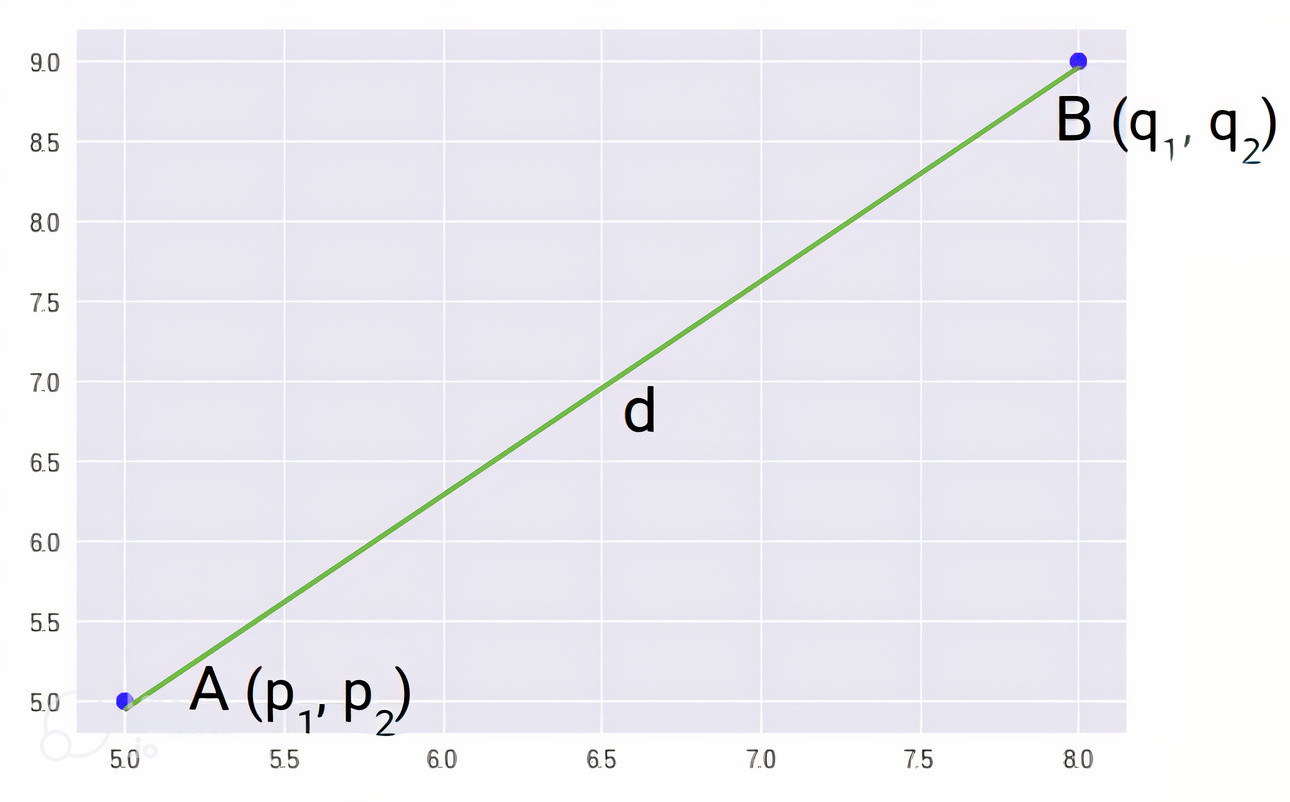
\includegraphics[width=0.75\linewidth]{figures/euclidean_distance}
	\caption{فاصله‌ی دو نقطه بر اساس فاصله‌ی اقلیدسی در دو بعد}\label{fig:euclidean_distance}
\end{figure}

\begin{equation} \label{d(p,q)}
	d\left( p,q\right) = \sqrt {\sum_{i=1}^{n} \left( q_{i}-p_{i}\right)^2 } 
\end{equation} 

\subsection{معیار فاصله‌ی ماهالانوبیس}
فاصله‌ی ماهالانوبیس\LTRfootnote[1]{Mahalanobis Distance}، فاصله‌ی بین دو نقطه در فضای چندمتغیره\LTRfootnote[2]{Multivariate Space} است. در یک فضای اقلیدسی منظم، متغیرها با محورهایی که در زوایای قائمه با یکدیگر ترسیم شده‌اند، نشان داده می‌شوند. فاصله‌ی بین هر دو نقطه را می‌توان با خط‌کش اندازه‌گیری کرد. برای متغیرهای غیر همبسته، فاصله‌ی اقلیدسی برابر با فاصله‌ی ماهالانوبیس است. با این ‌حال، اگر دو یا چند متغیر، همبسته باشند، محورها دیگر در زوایای قائم نیستند و اندازه‌گیری با یک خط‌کش غیرممکن می‌شود. علاوه بر این، اگر تعداد ابعاد بیشتر از سه باشد، دیگر در فضای سه‌ بعدی معمولی قابل ترسیم نخواهند بود. فاصله‌ی ماهالانوبیس، این مشکل اندازه‌گیری را حل می‌کند، زیرا فواصل بین نقاط را نسبت به یک مرکز اندازه‌گیری می‌کند. یک نقطه پایه یا مرکزی که می‌تواند به‌عنوان یک میانگین کلی برای داده‌های چند متغیره در نظر گرفته شود. هر چه فاصله‌ی ماهالانوبی بزرگ‌تر باشد، داده از مرکز دورتر است \cite{de2000mahalanobis}. نحوه‌ی محاسبه‌ی فاصله‌ی ماهالانوبیس در رابطه‌ی \ref{Delta} آمده است.\begin{figure}[h!]
	\centering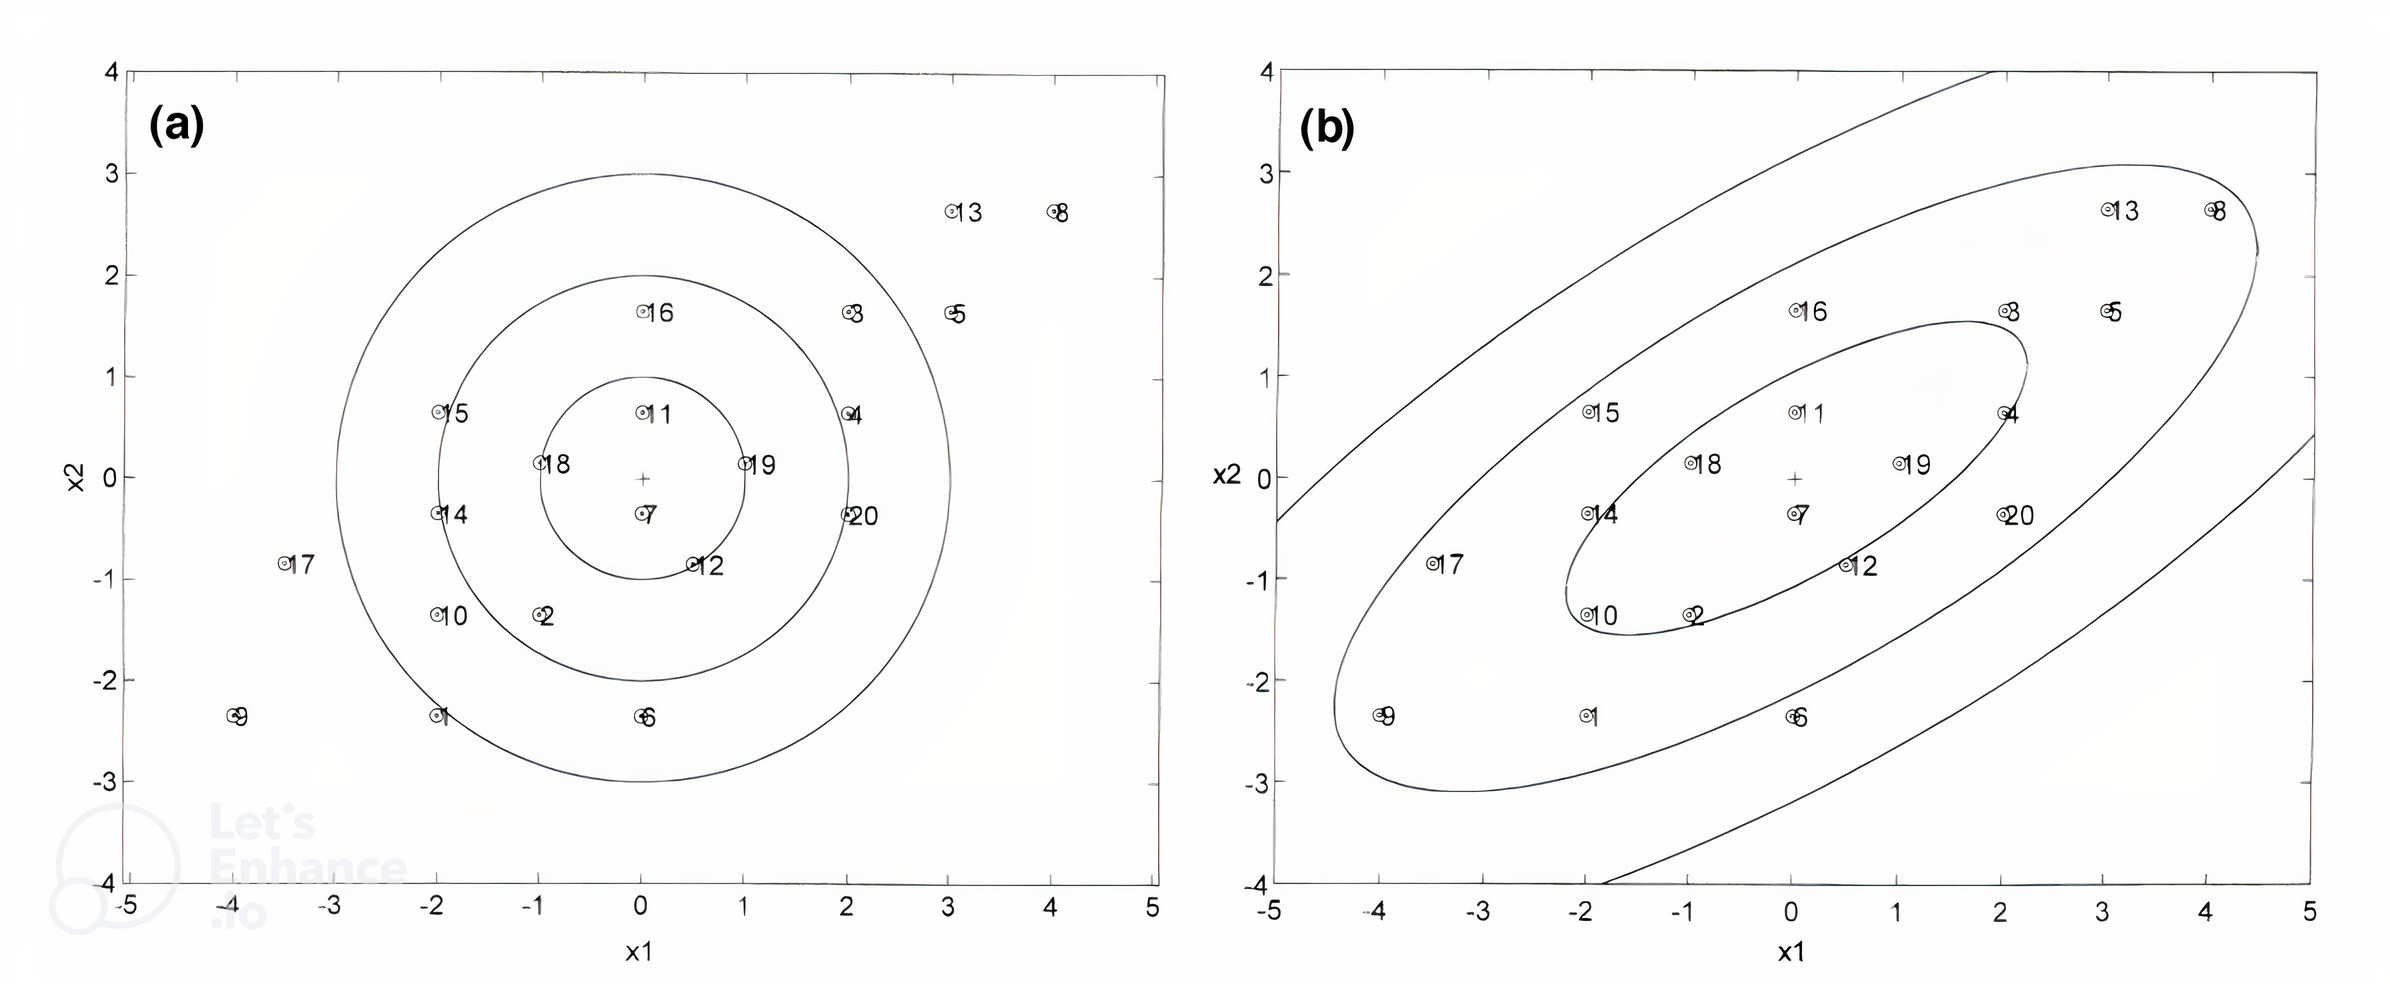
\includegraphics[width=1\linewidth]{figures/mahalanobis_figure}
	\caption{فاصله‌ی ماهالانوبیس حول یک نقطة مرکزی \cite{de2000mahalanobis}}\label{fig:mahalanobis_figure}
\end{figure} $\Sigma$ در فرمول زیر همان ماتریس کوواریانس است. در \cref{fig:mahalanobis_figure}، دو نمونه از محاسبه‌ی فاصله‌ی ماهالانوبیس برای تعدادی داده با دو متغیر \lr{x1} و \lr{x2} را مشاهده می‌کنید. همان‌طور که مشخص است فواصل تا یک نقطه‌ی مرکزی محاسبه شده است.  

\begin{equation} \label{Delta}
	\Delta^2 = \left( x-m\right)^\top\Sigma^{-1}\left( x-m\right)
\end{equation}

\subsection{خوشه‌بندی اقلیدسی}
خوشه‌بندی اقلیدسی\LTRfootnote{\lr{Euclidean Clustering}}، یک روش محبوب برای افراز یک ابر نقاط نامنظم به خوشه‌هایی کوچک‌تر است، که زمان لازم برای پردازش را به مراتب کاهش می‌دهد. این بازنمایی‌های خوشه‌ای، به فضای ابر نقاط نظم می‌دهند و برای زمانی که یک بازنمایی حجمی از فضای مسدود شده نیاز است، استفاده می‌شود. این روش برای زمانی که می‌خواهیم شکل اجسام تشخیص داده‌ شده در کادر محصورکننده را داشته باشیم نیز بسیار ارزشمند است. 

در عمل، برای پیدا کردن و بخش‌بندی\LTRfootnote{\lr{Segmentation}} خوشه اجسام متمایز،‌ معمولا از یک ساختار درخت کی‌دی\LTRfootnote{\lr{Kd-Tree}} استفاده می‌شود تا نزدیک‌‌ترین همسایه‌ها\LTRfootnote{\lr{Nearest Neighbours}} تشخیص داده شوند. الگوریتم این خوشه‌بندی به شکل زیر است:
\begin{enumerate}
    \item یک بازنمایی درخت کی‌دی برای ابر نقاط ورودی ساخته می‌شود $P$؛
    \item یک فهرست\LTRfootnote{List} از خوشه‌های خالی $C$ و یک صف\LTRfootnote{Queue} از نقاطی که بایستی بررسی شوند $Q$، ایجاد می‌شود؛
    \item به ازای هر نقطه $p_i \in P$، گام‌های زیر اجرا می‌شود:
    \begin{enumerate}
        \item نقطه $(p_i)$ را به صف اضافه کن؛
        \item به ازای هر نقطه $p_i \in Q$،‌ گام‌های زیر را انجام بده:
        \begin{itemize}
            \item در مجموعه نقاط همسایگی $P^k_i$، به دنبال نقاطی که در فاصله $r \l d_th$ هستند، جستجو کن؛
            \item به ازای هر همسایگی $p^k_i \in P^k_i$، بررسی کن که آیا نقطه قبلا پردازش شده است یا نه؛ اگر نه، آن را به صف $Q$ اضافه کن؛
        \end{itemize}
        \item زمانی که تمام نقاط داخل صف $Q$ پردازش شدند، $Q$ را به فهرست خوشه‌ها $C$ اضافه کن و $Q$ را خالی کن.
    \end{enumerate}
    \item الگوریتم زمانی خاتمه می‌یابد که تمام نقاط $p_i \in P$، پردازش شده باشند و عضو فهرست خوشه‌های $C$ شده باشند \LTRfootnote{\url{https://pcl.readthedocs.io/projects/tutorials/en/master/cluster_extraction.html}}.
\end{enumerate}

\subsection{مدل‌سازی سه‌بعدی}

مدل‌سازی سه‌بعدی هنر و علمی است که به ایجاد نمایش‌های دیجیتالی سه‌بعدی اجسام، صحنه‌ها یا محیط‌ها می‌پردازد. این تکنیک حیاتی در زمینه‌های مختلفی از جمله گرافیک کامپیوتری، انیمیشن، معماری، طراحی محصول و واقعیت مجازی به کار گرفته می‌شود. در دنیای مدل‌سازی سه‌بعدی، هنرمندان و طراحان از ابزارهای نرم‌افزاری ویژه برای ساخت مدل‌های سه‌بعدی با دقت و واقع‌گرایی بالا استفاده می‌کنند که قابلیت تغییر و مشاهده از زوایای مختلف را دارند. این مدل‌ها می‌توانند از اشکال هندسی ساده تا شخصیت‌های پیچیده، ساختارهای معماری یا جهان‌های مجازی کامل متغیر باشند. مدل‌سازی سه‌بعدی به عنوان پایه‌ای برای بسیاری از کاربردها عمل می‌کند و امکان ایجاد شخصیت‌های بازی ویدئویی واقع‌گرایانه، تصویرسازی طراحی‌های معماری، شبیه‌سازی پدیده‌های فیزیکی و بسیاری دیگر امکان‌پذیر می‌کند. با تنوع کاربردهای خود، مدل‌سازی سه‌بعدی نیرویی پیشرانه در عصر دیجیتال است که مرزهای خلاقیت و نوآوری را گسترش می‌دهد.

یکی از جنبه‌های کلیدی مدل‌سازی سه‌بعدی نمایش اجسام در فضای سه‌بعدی است، که معمولاً با استفاده از مختصات محورهای کارتزین تعریف می‌شود. این نمایش مکانی امکان ایجاد تجربیات جاذبه‌ای و تعاملی را فراهم می‌کند، زیرا مدل‌های سه‌بعدی می‌توانند برای شبیه‌سازی وضعیت‌های واقعی جهان، کاوش محیط‌های مجازی و انتقال اطلاعات پیچیده مورد استفاده قرار گیرند. برای مثال، توسعه شخصیت‌های واقع‌گرایانه برای فیلم‌های انیمیشنی، تجسم طراحی‌های معماری یا تجزیه و تحلیل داده‌های علمی، مدل‌سازی سه‌بعدی نقش اساسی در احیای ایده‌ها و مفاهیم در دنیای دیجیتال ایفا می‌کند. با پیشرفت فناوری، تکنیک‌های مدل‌سازی سه‌بعدی نیز تکامل می‌کنند و فرصت‌های جدیدی برای خلاقیت و حل مسائل در صنایع مختلف ارائه می‌دهند.

\begin{figure}[h]
    \centering
    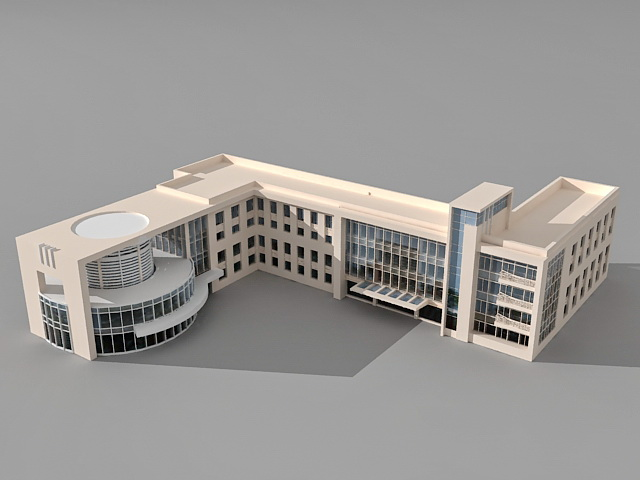
\includegraphics[width=0.7\linewidth]{3D_Model.png}
    \caption{مدل سه‌بعدی یک ساختمان}
    \label{fig:3D_Model}
\end{figure}


\section{نگاهی بر کار‌های پیشین}

در این بخش نگاهی مختصر به پژوهش‌هایی می‌اندازیم که علم دوقلوهای دیجیتال و نحوه ساختن آن را به چالش می‌کشند.

\subsection{طراحی سیستماتیک دوقلوی دیجیتال}

تحقیقات گوناگونی در زمینه طراحی سیستماتیک دوقلوی دیجیتال وجود دارند. در سال 2019، گروهی از محققین دانشگاه کمبریج\LTRfootnote{\lr{University of Cambridge}} اقدام به ساخت دوقلوی دیجیتالی از پردیس غربی کمبریج کردند \cite{lu2020developing}. در این مقاله، تمرکز اصلی بر روی عقب بودن عمران، معماری و مدیریت سازه\LTRfootnote{\lr{AEC/FM}} از تکنولوژی و عدم بکارگیری دوقلوهای دیجیتالی برای پیاده‌سازی پروژه‌های ساختمانی است. در این مقاله آمده است که در سال 2017، دولت بریتانیا پیشنهادی مبتنی بر ساختن دوقلوی دیجیتالی از کشور مطرح کرد و طبق گزارش‌های منتشر شده، این اقدام نیازمند آن است که شرکت‌های عمرانی و معماری، دوقلوی دیجیتال سازه‌های خود را تهیه نمایند. برای پیاده‌سازی دوقلوی دیجیتال از یک کشور، بایستی از هزاران دوقلوی دیجیتالی کوچک‌تر مانند دوقلوی دیجیتالی شهری و ساختمانی و جاده‌ای بهره برد. در ادامه شکل 1-2 از نحوه شکل‌گیری دوقلوی دیجیتالی برای یک کشور آورده شده است:

\begin{figure}[h]
	\centering
	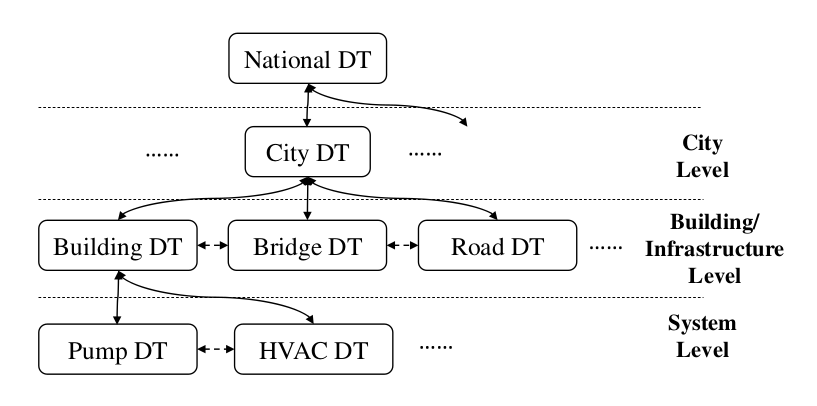
\includegraphics[scale=0.4]{figures/DT connections and hierarchy among different levels.png}
	\caption{  معماری دوقلوهای دیجیتالی و سلسله مراتب آنها \cite{lu2020developing}}
	\label{fig:dt_connections_and_hierarchy}
\end{figure}

با توجه به \cref{fig:dt_connections_and_hierarchy}، می‌توان دریافت کرد که دوقلوی‌ دیجیتال یک مجموعه بزرگ مانند کشور یا شهر، از دوقلو‌های دیجیتال کوچک‌تری شکل گرفته است. این مقاله به طراحی دوقلوی دیجیتال در ابعاد کوچک می‌پردازد که راه و روش‌های ایجاد دوقلوی دیجیتال پردیس دانشگاه را بررسی می‌کند.
این مقاله، اولین مقاله‌ای است که به طور سیستماتیک ساختن یک مدل از پردیس دانشگاه را انجام داده است و مراحل طراحی و معماری دوقلوی دیجیتال خود را به ساختن یک شهر یا کشور دیجیتالی براساس مقاله‌های گوناگون تعمیم داده است و تمامی محققان را در بکارگیری از این معماری تشویق کرده‌ است. 

\subsection{نحوه‌ی بهینه‌ مدل‌سازی سه‌بعدی دوقلوهای دیجیتال}

در مقاله‌‌ای دیگر که در سال ۲۰۲۲ توسط محققین دانشگاه تگزاس ال پاسو\LTRfootnote{\lr{University of Texas El Paso}} منتشر شده است،‌ یک روش عملی و کارآمد برای ایجاد دوقلوی دیجیتال هر مکان جغرافیایی، بخصوص دوقلوی دیجیتال دانشگاه‌ها و شبکه‌ی جاده‌ها معرفی شده است \cite{azfar2022efficient}. نویسندگان این مقاله، به چالش‌هایی که محققین گوناگون در ایجاد مدل‌های سه‌بعدی دقیق روبه‌رو می‌شوند را مورد تاکید کرده است و اهمیت تصویرسازی و شبیه‌سازی در تحقیقات دوقلوهای دیجیتال را بیان می‌کنند. آن‌ها یک جریان کاری ارائه می‌دهند که از داده‌ سرویس ‌\lr{OSM}\LTRfootnote{\lr{OpenStreetMap}} به عنوان پایه برای مدل‌سازی شبکه‌های جاده استفاده می‌کند و روشی برای ادغام اطلاعات زمینه‌ای مانند ساختمان‌ها و پستی بلندی\LTRfootnote{\lr{Terrain}} ارائه می‌دهد. این مقاله در مورد کاربرد‌های این روش در حوزه‌های مختلف همانند طراحی شبکه‌های جاده، شبیه‌سازی‌ خودرو‌های خودران با ابزار‌هایی مانند سومو\LTRfootnote{\lr{SUMO}} و کارلا\LTRfootnote{\lr{CARLA}} و  بخصوص در مورد تحقیقات بینایی کامپیوتر\LTRfootnote{\lr{Computer Vision}}  در محیط‌های دیجیتال و مصنوعی صبحت می‌کند. سپس این مقاله با برجسته کردن قابلیت چند‌منظوره بودن، مقیاس‌ پذیری و انعطاف پذیری روش پیشنهادی برای تحقیقات مختلف به پایان می‌رسد. این مقاله تاکید می‌کند که این رویکرد برای مدل‌سازی، شبیه‌سازی و تصویر‌سازی سه‌بعدی، بهره‌وری و کارآمدی دارد در حیطه‌های مختلف مانند حمل‌ و نقل، زیرساخت و بینایی کامپیوتر مفید و مقرون به صرفه است.

\begin{figure}[h]
	\centering
	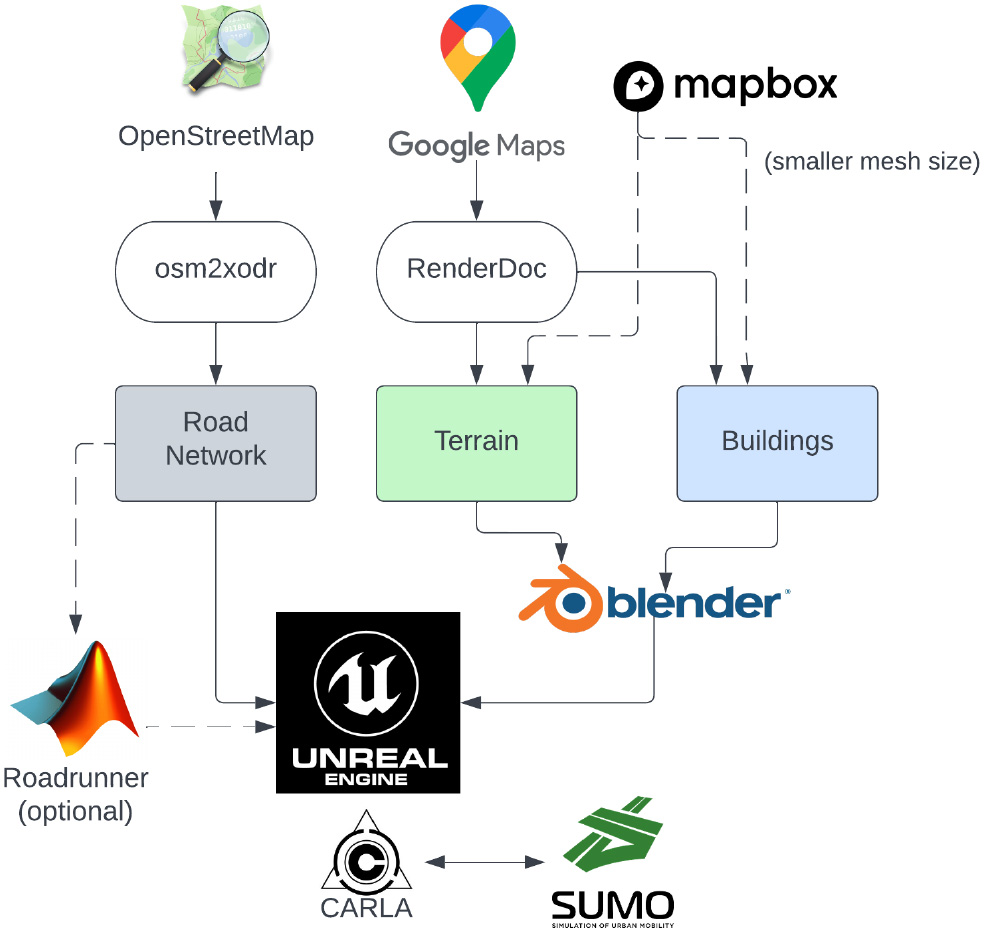
\includegraphics[scale=0.24]{figures/Digital_Twin_Procedure.png}
	\caption{  خلاصه‌ای از روش پیشنهاد شده برای ایجاد دوقلوی دیجیتال یک منطقه (در فصل چهارم به تحلیل دقیق این شکل می‌پردازیم) \cite{azfar2022efficient}}
	\label{fig:dt_procedure}
\end{figure}

\subsection{چرخه‌ی شبیه‌سازی خودکار اجسام پویا در دوقلوهای دیجیتال}

مقاله‌‌‌های دیگری نیز در زمینه تولید خودکار دوقلوی دیجیتال از یک جاده وجود دارند. مقاله‌‌ای در سال 2022 منتشر شده است که در زمینه ساخته شدن خودکار مدل‌های دوقلوی دیجیتالی صحنه‌های ترافیکی تحقیق می‌کند \cite{wang2022automatic}. در این مقاله با استفاده از حسگرهای لایدار و ابر نقاط، محیط اطراف با استفاده از خوشه بندی با مقیاس فاصله اقلیدسی\LTRfootnote{\lr{Euclidean Clustering}} دسته‌بندی می‌شود و براساس داده‌های پردازش شده از خوشه‌‌ها، دوقلوی دیجیتال ساخته می‌شود. \cref{fig:automatic_dt_creation_cycle} مراحل طی شده برای شکل‌گیری خودکار دوقلوی دیجیتال را نشان می‌دهد.

\begin{figure}[h]
	\centering
	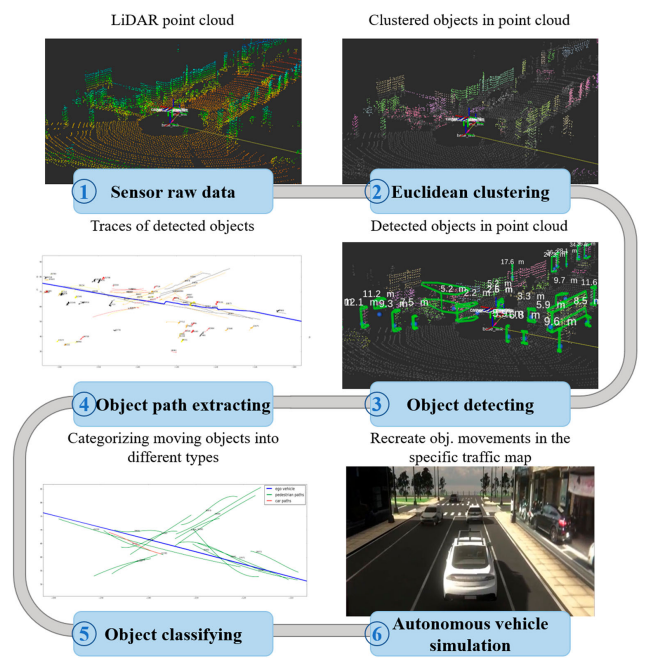
\includegraphics[scale=0.87]{figures/Automatic_DT_Creation_Cycle.png}
	\caption{  چرخه پردازش داده و تشخیص پارامترهای پویا و ساختن دوقلوی دیجیتال به صورت خودکار \cite{wang2022automatic}}
	\label{fig:automatic_dt_creation_cycle}
\end{figure}

حال به شرح هر کدام از بخش‌های \cref{fig:automatic_dt_creation_cycle} می‌پردازیم:
\begin{enumerate}
    \item برداشت اطلاعات سه بعدی از حسگر لایدار و ارسال اطلاعات در فرمت ابر نقاط به سرور
    \item از الگوریتم خوشه‌بندی با مقیاس فاصله اقلیدسی بر روی ابر نقاط برای تشخیص اجسام استفاده می‌شود. همچنین شناسه‌ای برای هر خوشه تشخیص داده شده در نظر گرفته می‌شود تا در مراحل بعدی جهت حرکت اجسام تشخیص داده شود.
    \item با استفاده از الگوریتم‌های تشخیص اجسام براساس کادر محصورکننده خوشه‌ها\LTRfootnote{\lr{Bounding-Box Based Detection Algorithms}}، اجسام خوشه‌بندی شده برچسب‌ گذاری می‌شوند و اجسامی که کادر محصورکننده آن‌ها بیشتر از کمینه تعیین شده توسط الگوریتم نباشد فیلتر می‌شوند (به علت‌های گوناگون ممکن است خوشه‌هایی وجود داشته باشد که شئ واقعی نباشند). همچنین جهت قرارگیری جسم، ثابت یا متحرک بودن جسم و جهت حرکت جسم تشخیص داده می‌شود.
    \item محاسبه مسیر حرکتی اجسام تشخیص داده‌ شده با تعیین موقعیت آن جسم در طول زمان
    \item دسته‌بندی اجسام براساس اندازه کادر محصورکننده به دسته‌های خودرو، موتورسیکلت و عابر پیاده
    \item پارامترهای گوناگون تشخیص داده شده در مراحل قبل بایستی پردازش شوند و مختصات و مسیر‌های حرکت اجسام تشخیص داده شده، به مختصات مدل سه بعدی شبیه‌سازی، تبدیل بشوند. در نهایت نیز مدل‌های سه بعدی اجسام براساس نوع آن جسم در نقشه مدل سه‌بعدی شبیه‌سازی با توجه به مختصاتشان قرار داده ‌می‌شوند و براساس مسیر حرکت خود، شروع به حرکت می‌کنند. حال می‌توان سیستم‌های ماشین‌ خودران را در این بستر ایجاد شده آزمود.
\end{enumerate}

مشاهده کردیم که هر کدام از مقالات، به دنبال مطرح کردن روشی سیستماتیک برای پیاده‌سازی دوقلو‌های دیجیتال هستند. همچنین مشاهده کردیم که در سال ۲۰۲۲ تحقیقاتی در زمینه خودکار کردن این پروسه صورت گرفته است. این پایان‌نامه نیز با الهام گیری از مقالات فوق، اقدام به پیاده‌سازی دوقلویی دیجیتال کرده است.